%File principale del documento su cui invocare la compilazione, vedi "istruzioni.txt" per più info

%Preambolo: la parte prima del \begin{document}
\documentclass[12pt,a4paper]{article} %formato del documento e grandezza caratteri

%Input del file metadata.tex della cartella locale "res/"
%lista di comandi presenti in template_latex.tex, da qui posso essere modificati secondo le esigenze

\newcommand{\DocTitle}{Verbale interno 2019-11-18} %variabile usata dal file template_latex.tex per settare il titolo del documento
%\newcommand{\DocAuthor}{Progetto "Predire in Grafana"} %variabile usata dal file template_latex.tex per settare l'autore del documento
\newcommand{\DocDate}{18 Novembre 2019} %variabile usata dal file template_latex.tex; Impostata manualmente, altrimenti ad ogni compilazione viene messa la data del giorno di compilazione.
\newcommand{\DocDesc}{Resoconto dell'incontro del gruppo \textit{VRAM Software} tenutosi in data 2019-11-18} %variabile usata dal file template_latex.tex per settare la descrizione del documento
\newcommand{\ver}{27.0.0} %variabile usata dal file template_latex.tex per settare la versione del documento
\newcommand{\app}{Toffoletto Massimo} %variabile usata dal file template_latex.tex per settare l'approvatore del documento
\newcommand{\red}{Dalla Libera Marco} %variabile usata dal file template_latex.tex per settare il redattore del documento
\newcommand{\test}{Schiavon Rebecca} %variabile usata dal file template_latex.tex per settare il verificatore del documento
\newcommand{\stat}{Approvato} %variabile usata dal file template_latex.tex per settare lo stato del documento
\newcommand{\use}{Interno} %variabile usata dal file template_latex.tex per indicare l'uso del documento %Contiene le varibili che descrivono il documento

%Input di file di configurazione presi dalla cartella "Template-LaTeX/config/", uguali per tutti i documenti
%Attenzione bisogna impostare il percorso del file!
% Tutti i pacchetti usati, da inserire nel preambolo prima delle configurazioni

\usepackage[T1]{fontenc} %Permette la sillabazione su qualsiasi testo contenente caratteri
\usepackage[utf8]{inputenc} %Serve per usare la codifica utf-8
\usepackage[english,italian]{babel} %Imposta italiano lingua principale, inglese secondaria. Es. serve per far apparire "indice" al posto di "contents"

\usepackage{graphicx} %Serve per includere le immagini

\usepackage[hypertexnames=false]{hyperref} %Gestisce i riferimenti/link. Es. Serve per rendere clickabili le sezioni dell'indice

\usepackage{float} %Serve per migliore la definizione di oggetti fluttuanti come figure e tabelle. Es. poter usare l'opzione [H] nelle figure ovvero tenere fissate le immagini che altrimenti LaTeX si sposta a piacere.

\usepackage{listings} %Serve per poter mettere snippets di codice nel testo

\usepackage{lastpage} %Serve per poter introdurre un'etichetta a cui si può fare riferimento Es. piè di pagina; poter fare " \rfoot{\thepage\ di \pageref{LastPage}} "

\usepackage{fancyhdr} %Per header e piè di pagina personalizzati

%Sono alcuni package che potranno esserci utili in futuro
%\usepackage{charter}
%\usepackage{eurosym}
\usepackage{subcaption}
%\usepackage{wrapfig}
%\usepackage{background}
\usepackage{longtable} % tabella che può continuare per più di una pagina
\usepackage[table]{xcolor} % ho dovuto aggiungere table in modo da poter colorare le row della tabella, dava: undefined control sequences
%\usepackage{colortbl}

\usepackage{dirtree} % usato per creare strutte tree-view in stile filesystem
\usepackage{xspace} % usato per inserire caratteri spazio
\usepackage[official]{eurosym}
\usepackage{pdflscape} %Inclusione pacchetti
% Configurazioni varie, da inserire nel preambolo dopo i pacchetti

\hypersetup{hidelinks} %serve per nascondere riquadri rossi che circondano i link 

\lstset{literate= {à}{{\`a}}1 } %Permette di usare lettere accentate nei listings

\pagestyle{fancy} %Imposto stile pagina
\fancyhf{} %Reset, se lo tolgo LaTex mette impostazioni di default (p.es numerazione pagine di default)


\lhead{
\includegraphics[scale=0.25]{img/logo_header.png}} %Left header che compare in ogni pagina
%\rhead{\leftmark} %Nome della top-level structure (p.es. Section in article o Chapter in book) in ogni pagina
\rhead{\DocTitle\ v. \ver} %Right header

\newcommand{\glo}{$_G$} %Comando per aggiungere il pedice G
\newcommand{\glosp}{$_G$ } %Comando per aggiungere il pedice G con spazio

\newcommand\Tstrut{\rule{0pt}{2.6ex}} % top padding
\newcommand\Bstrut{\rule[-0.9ex]{0pt}{0pt}} % bottom padding
\newcommand{\TBstrut}{\Tstrut\Bstrut} % top & bottom padding

%Setto il colore dei link
%\hypersetup{
%	colorlinks,
%	linkcolor=[HTML]{404040},
%	citecolor={purple!50!black},
%	urlcolor={blue!50!black}
%}

%Tabelle e tabulazione (può tornare utile)
%\setlength{\tablcolsep}{10pt}
%\renewcommand{\arraystretch}{1.4}

%Comando per aggiungere le pagine di ogni sezione
%\newcommand{\newSection}[1]{%
%	\input{res/sections/#1}
%}

% Comandi per aggiungere padding a parole contenute nella tabella; è una specie di strut (un carattere invisibile)
%\newcommand\Tstrut{\rule{0pt}{2.6ex}} % top padding
%\newcommand\Bstrut{\rule[-0.9ex]{0pt}{0pt}} % bottom padding
%\newcommand{\TBstrut}{\Tstrut\Bstrut} % top & bottom padding  %Configurazione pacchetti

\begin{document}
	%Input del file "frontmatter" preso dalla cartella "Template-LaTeX/config/", uguale per tutti i documenti
	%Attenzione bisogna impostare il percorso del file!
	% #### FRONTESPIZIO (frontmatter) ####
\setlength{\headheight}{33pt} %Distanzia l'header
\pagenumbering{gobble} %Toglie il numero di pagina
\begin{titlepage}
	\begin{center}
		
\includegraphics[scale=0.6]{img/logo.png} \\ %Logo
		\vspace{0.4cm} %Aggiunge uno spazio verticale di 0.5 cm
		
		{\LARGE Progetto "Predire in Grafana"} \\ %Nome progetto
		\vspace{0.4cm} %Attenzione a mettere il punto e NON la virgola
		
		{\Huge \textbf{\DocTitle}} \\ %Titolo, prende variabile definita in metadata.tex
		\vspace{0.4cm}
		
		\DocDate \\ %Data, prende variabile definita in metadata.tex
		\vspace{0.4cm}
		
		%Allineamento colonne: l=left r=right c=center, 
		%va specificato per ogni colonna
		%Se si vuole la riga tra colonne mettere "|"
		
		\begin{tabular}{r | l} %Elementi colonne separate da "&", le righe finiscono con "\\"
			Versione             & \ver \\
			Approvazione         & \app \\ 
			Redazione            & \red \\
			Verifica             & \test \\
			Stato                & \stat \\
			Uso                  & \use \\
		    Destinato a          & Zucchetti \\
						         & Prof. Vardanega Tullio\\
						         & Prof. Cardin Riccardo\\
			Email di riferimento & vram.software@gmail.com
		\end{tabular}
		\vfill
		\textbf{Descrizione} \\
		\DocDesc
	\end{center}
\end{titlepage}
\clearpage

% #### Impostazione header, footer  e numerazione pagine ####
\pagenumbering{arabic} %Pagine con i numeri arabi + reset a 1
\renewcommand{\footrulewidth}{0.4pt} %Di default footrulewidth==0 e quindi è invisibile, di default \headrulewith==0.4pt
\rfoot{\thepage\ di \pageref{LastPage}} %Pagina n di m, con numeri Arabi; usa il pacchetto "lastpage", in caso non sia possibile usare tale pacchetto mettere al fondo dell'ultima pagina "\label{LastPage}"

% #### Tabella dei log ####
% \textbf = grassetto; \Large = font più grande
% \rowcolors{quanti colori alternare}{colore numero riga pari}{colore numero riga dispari}: colori alternati per riga
% \rowcolor{color}: cambia colore di una riga
% p{larghezza colonna}: p è un tipo di colonna di testo verticalmente allineata sopra, ci sarebbe anche m che è centrata a metà ma non è precisa per questo utilizzo TBStrut; la sintassi >{\centering} indica che il contenuto della colonna dovrà essere centrato
% \TBstrut fa parte di alcuni comandi che ho inserito in config.tex che permetto di aggiungere un po' di padding al testo
% \\ [2mm] : questra scrittura indica che lo spazio dopo una break line deve essere di 2mm
% 

%\setcounter{secnumdepth}{0}
%\hfill \break
%\textbf{\Large{Diario delle modifiche}} \\


\addtocontents{toc}{\protect\setcounter{tocdepth}{0}} %Inserire questo per escludere una sezione dall'indice.

\section*{Registro delle modifiche} %Asterisco per fare sezione non numerata
\rowcolors{2}{gray!25}{gray!15}
\begin{longtable} {
		>{\centering}p{17mm} 
		>{\centering}p{19.5mm}
		>{\centering}p{24mm} 
		>{\centering}p{24mm} 
		>{}p{32mm}}
	\rowcolor{gray!50}
	\textbf{Versione} & \textbf{Data} & \textbf{Nominativo} & \textbf{Ruolo} & \textbf{Descrizione} \TBstrut \\
	14.7.0 & 2020-04-09 & Stantagiuliana Vittorio, Toffoletto Massimo e Spreafico Alessandro & \textit{Progettista}, \textit{Verificatore} e \textit{Responsabile di progetto} & Stesura, verifica e approvazione documento. \TBstrut \\ [2mm]
\end{longtable}

\addtocontents{toc}{\protect\setcounter{tocdepth}{4}} %Inserire questo per ripristinare il normale inserimento delle sezioni nell'indice. 4 significa fino al paragrah
\clearpage

% #### INDICE (tableofcontents) ####
\tableofcontents %Provoca la stampa dell'indice
\clearpage

\setcounter{secnumdepth}{4} %Permette di andare fino alla profondità del paragraph con la numerazione delle sezioni %Imposta il frontespizio, l'indice, header e footer
	
	\listoftables
	\pagebreak
	\listoffigures
	\pagebreak
	
	\section{Introduzione}
	\subsection{Premessa}
	Il Piano di Qualifica è un documento che sarà ampliato incrementalmente con il proseguimento del progetto\glo, non è quindi da considerarsi completo. Questo modus operandi è supportato dall'adesione al modello a V\glo, secondo il quale nel periodo di analisi si può procedere alla stesura dei soli test di accettazione e di sistema.
	
	\subsection{Scopo del documento}
	Il compito del \textit{Piano di Qualifica} è fissare quantitativamente, tramite valori soglia o intervalli, gli obiettivi di qualità di prodotto\glosp e di processo\glosp assunti nel progetto\glo. Inoltre utilizza le metriche\glosp definite nel documento \textit{Norme di Progetto} specificando le modalità con cui viene verificato il raggiungimento.

	\subsection{Scopo del prodotto}
	Lo scopo del prodotto\glosp è creare un plug-in di Grafana\glosp che usi dei modelli di predizione per produrre dei valori aggiunti al flusso del monitoraggio come se fossero stati rilevati dal campo. Insieme al plug-in viene sviluppato un programma per la gestione dei parametri degli algoritmi di previsione, che permette di allenare gli algoritmi con dei dati di test. Il fine del plug-in è monitorare la "liveliness" del sistema a supporto dei processi DevOps\glosp e di consigliare interventi nel sistema di produzione del software.
	
	\subsection{Glossario}
	I termini ambigui e bisognosi di spiegazione presenti in questo documento, contrassegnati da una 'G' a pedice, sono chiariti nel \textit{Glossario v. 1.1.1}.
	
	\subsection{Riferimenti}
		\subsubsection{Riferimenti normativi}
		\begin{enumerate}
			\item \textbf{Norme di Progetto}: \textit{Norme di Progetto v. 1.1.1};
			\item \textbf{Capitolato}\glosp \textbf{d'appalto C4 - Predire in Grafana}\glo: \url{https://www.math.unipd.it/~tullio/IS-1/2019/Progetto/C4.pdf}.
		\end{enumerate}
	
		\subsubsection{Riferimenti informativi}
		\begin{enumerate}
		    \item \textbf{Modello a V}: \url{https://www.math.unipd.it/~tullio/IS-1/2019/Dispense/L14.pdf}.
		\end{enumerate}
	
	
	

	
	
	
	

	\pagebreak
	\section{Qualità di processo}
Per misurare la qualità di processo\glosp il gruppo ha definito degli obiettivi di qualità e delle metriche\glosp che li rendano quantificabili prendendo come riferimento le norme della serie ISO 9000. Tali norme definiscono i requisiti per la realizzazione di un sistema di gestione della qualità, al fine di ottenere dei processi\glosp efficaci ed efficienti.
	\subsection{PRC-Q2 Processo di sviluppo}
		\subsubsection{OP-1 Individuazione completa dei requisiti} 
			Ci prefiggiamo individuare in modo corretto e completo i requisiti sin da subito per evitare modifiche che comportano un grosso dispendio di tempo.
			\paragraph{Metriche di qualità} \mbox{}
			\rowcolors{2}{gray!25}{gray!15}
			\begin{longtable} {
					>{}p{80mm} 
					>{}p{25mm}
					>{}p{25mm}
				}
				\rowcolor{gray!50}
				\textbf{Metrica} & \textbf{Preferibile} & \textbf{Accettabile} \TBstrut \TBstrut \\
				M01 Scostamento dei requisiti individuati & 0 & $\le 10$ \TBstrut \\ [2mm]
			\end{longtable}
			
		\subsubsection{OP-2 Sviluppo di codice comprensibile e manutenibile}
			Ci prefiggiamo di scrivere codice che segua le norme di codifica indicate nelle \textit{Norme di Progetto} e sia manutenibile nel tempo, al fine di garantire comprensibilità e manutenibilità del codice.
			\paragraph{Metriche di qualità} \mbox{}
			\begin{longtable} {
					>{}p{80mm} 
					>{}p{25mm}
					>{}p{25mm}
				}
				\rowcolor{gray!50}
				\textbf{Metrica} & \textbf{Preferibile} & \textbf{Accettabile} \TBstrut \TBstrut \\
				M02 Numero di parametri per metodo & $ \le 3$ & $ \le 5$ \TBstrut \\ [2mm]
				M03 Numero di metodi per classe & $ \le 8$ & $ \le 15$ \TBstrut \\ [2mm]
				M20 Livello di annidamento & $1 \le x \le 3$ & $1 \le x \le 7$ \TBstrut \\ [2mm]
			\end{longtable}
	
		\subsubsection{OP-9 Forte disaccoppiamento tra le componenti architetturali}
		Ci prefiggiamo di progettare l'architettura del prodotto\glosp software con un forte disaccoppiamento tra le componenti in modo che sia efficace, efficiente e facilmente manutenibile;
		\paragraph{Metriche di qualità} \mbox{}
		\rowcolors{2}{gray!25}{gray!15}
		\begin{longtable} {
				>{}p{80mm} 
				>{}p{25mm}
				>{}p{25mm}
			}
			\rowcolor{gray!50}
			\textbf{Metrica} & \textbf{Preferibile} & \textbf{Accettabile} \TBstrut \TBstrut \\
			M21 Profondità della gerarchia & $\le 4$ & $\le 7$ \TBstrut \\ [2mm]
			M22 Numero di design pattern & $5 \le x \le 6$ & $2 \le x \le 15$ \TBstrut \\ [2mm]
		\end{longtable}
			
	\subsection{PRC-Q5 Processo di garanzia della qualità}
		\subsubsection{OP-3 Monitoraggio della qualità}
			Ci prefiggiamo di monitorare la qualità dei processi\glosp e dei prodotti\glosp al fine di ottenere un controllo e un miglioramento continuo. 
			\paragraph{Metriche di qualità} \mbox{} 
			\begin{longtable} {
					>{}p{80mm} 
					>{}p{25mm}
					>{}p{25mm}
				}
				\rowcolor{gray!50}
				\textbf{Metrica} & \textbf{Preferibile} & \textbf{Accettabile} \TBstrut \TBstrut \\
				M04 Percentuale di metriche soddisfatte & $100\%$ & $\ge 60\%$ \TBstrut \\ [2mm]
			\end{longtable}

	\subsection{PRC-Q6 Processo di verifica}
		\subsubsection{OP-4 Efficacia dei test}
			Ci prefiggiamo di svolgere una verifica efficace su ogni parte del nostro prodotto\glo.
			\paragraph{Metriche di qualità} \mbox{}
			\begin{longtable} {
					>{}p{80mm} 
					>{}p{25mm}
					>{}p{25mm}
				}
				\rowcolor{gray!50}
				\textbf{Metrica} & \textbf{Preferibile} & \textbf{Accettabile} \TBstrut \TBstrut \\
				M05 Percentuale bug sistemati & $100\%$ & $100\%$ \TBstrut \\ [2mm]
			\end{longtable}
		\subsubsection{OP-5 Completezza dei test}
		Ci prefiggiamo di svolgere una verifica completa su ogni parte del nostro prodotto\glo.
		\paragraph{Metriche di qualità} \mbox{}
		\begin{longtable} {
				>{}p{80mm} 
				>{}p{25mm}
				>{}p{25mm}
			}
			\rowcolor{gray!50}
			\textbf{Metrica} & \textbf{Preferibile} & \textbf{Accettabile} \TBstrut \TBstrut \\
			M23 Code coverage & $100\%$ & $\ge 80\%$ \TBstrut \\ [2mm]
			M24 Branch coverage & $100\%$ & $\ge 80\%$ \TBstrut \\ [2mm]
			M25 Copertura dei test eseguiti & $\ge 90\%$ & $100\%$ \TBstrut \\ [2mm]
		\end{longtable}	
			
	\subsection{PRC-Q8 Processo di gestione dei cambiamenti}
		\subsubsection{OP-6 Risoluzione efficace dei problemi}
			Ci prefiggiamo di gestire ogni cambiamento necessario in tempi ragionevolmente brevi.
			\paragraph{Metriche di qualità} \mbox{}			
			\begin{longtable} {
					>{}p{80mm} 
					>{}p{25mm}
					>{}p{25mm}
				}
				\rowcolor{gray!50}
				\textbf{Metrica} & \textbf{Preferibile} & \textbf{Accettabile} \TBstrut \TBstrut \\
				M06 Tempo medio risoluzione errori & $\le 10$ minuti & $\le 120$ minuti \TBstrut \\ [2mm]
			\end{longtable}					

	\subsection{PRC-Q9 Processo di gestione organizzativa}
		\subsubsection{OP-7 Pianificazione efficace delle risorse}
			Ci prefiggiamo di rispettare le tempistiche e i costi indicati nel preventivo nel documento \textit{Piano di Progetto}.
			\paragraph{Metriche di qualità} \mbox{} 
			\begin{longtable} {
					>{}p{60mm} 
					>{}p{35mm}
					>{}p{50mm}
				}
				\rowcolor{gray!50}
				\textbf{Metrica} & \textbf{Preferibile} & \textbf{Accettabile} \TBstrut \TBstrut \\
				M07 Planned Value & $\ge$ 0 & $\ge$ 0 \TBstrut \\ [2mm]
				M08 Earned Value & = PV & $\ge$ 0 \TBstrut \\ [2mm]
				M09 Actual cost & 0 $\le$ AC $\le$ PV &0 $\le$ AC $\le$ budget totale \TBstrut \\ [2mm]				
				M10 Cost Performance Index & 1 & 0.95 $\le$ CPI $\le$ 1.05 \TBstrut \\ [2mm]				
				M11 Schedule Performance Index & 1 & 0.95 $\le$ SPI $\le$ 1.05 \TBstrut \\ [2mm]				
				M12 Estimated Cost at Completion & quanto preventivato & preventivo-5\% $\le$ EAC $\le$ preventivo+5\% \TBstrut \\ [2mm]
				M13 Schedule at Completion & quanto preventivato & quanto preventivato \TBstrut \\ [2mm]				
			\end{longtable}

		\subsubsection{OP-8 Prevenzione dei rischi} 
			Ci prefiggiamo di individuare fin da subito i rischi in modo completo per evitare il cambiamento degli stessi nel tempo e prevenirli.
			\paragraph{Metriche di qualità} \mbox{} 
			\begin{longtable} {
					>{}p{80mm} 
					>{}p{25mm}
					>{}p{25mm}
				}
				\rowcolor{gray!50}
				\textbf{Metrica} & \textbf{Preferibile} & \textbf{Accettabile} \TBstrut \TBstrut \\
				M14 Rischi non preventivati & 0 & $ \le 5$ \TBstrut \\ [2mm]
			\end{longtable}
			

	\subsection{Tabella riassuntiva delle metriche adottate}
	\rowcolors{2}{gray!25}{gray!15}
	\begin{longtable} {
		>{}p{50mm}  
		>{}p{80mm}
		}

		\rowcolor{gray!50}
		\multicolumn{2}{c}{\textbf{PRC-Q1 Processo di sviluppo}}\\
	\rowcolor{gray!50}
	\textbf{Obiettivi} & \textbf{Metriche} \TBstrut \\ [2mm]

		OP-1 Individuazione completa dei requisiti &
		M01 Scostamento dei requisiti individuati \TBstrut \\ [2mm]

		OP-2 Sviluppo di codice comprensibile e manutenibile &
		M20 Livello di annidamento \newline
		M02 Numero di parametri per metodo \newline
		M03 Numero di metodi per classe \TBstrut \\ [2mm]
		
		OP-9 Forte disaccoppiamento tra le componenti architetturali &
		M21 Profondità della gerarchia \newline
		M22 Numero di design pattern \TBstrut \\ [2mm]

		\rowcolor{gray!50}
		\multicolumn{2}{c}{\textbf{PRC-Q2 Processo di garanzia della qualità}}\\
	\rowcolor{gray!50}
	\textbf{Obiettivi} & \textbf{Metriche} \TBstrut \\ [2mm]

		OP-3 Monitoraggio della qualità &
		M04 Percentuale di metriche soddisfatte \TBstrut \\ [2mm]
		
	\rowcolor{gray!50}
	\multicolumn{2}{c}{\textbf{PRC-Q3 Processo di verifica}}\\
	\rowcolor{gray!50}
	\textbf{Obiettivi} & \textbf{Metriche} \TBstrut \\ [2mm]

		OP-4 Efficacia dei test &
		M05 Percentuale bug sistemati \TBstrut \\ [2mm]
		OP-5 Completezza dei test & 
		M23 Code coverage \newline
		M24 Branch coverage \newline
		M25 Copertura dei test eseguiti \TBstrut \\ [2mm]

	\rowcolor{gray!50}
	\multicolumn{2}{c}{\textbf{PRC-Q4 Processo di gestione dei cambiamenti}}\\
	\rowcolor{gray!50}
	\textbf{Obiettivi} & \textbf{Metriche} \TBstrut \\ [2mm]

		OP-6 Risoluzione efficace dei problemi &
		M06 Tempo medio risoluzione errori \TBstrut \\ [2mm]

	\rowcolor{gray!50}
		\multicolumn{2}{c}{\textbf{PRC-Q5 Processo di gestione organizzativa}}\\
	\rowcolor{gray!50}
		\textbf{Obiettivi} & \textbf{Metriche} \TBstrut \\ [2mm]

		OP-7 Pianificazione efficace delle risorse & 
		M07 Planned Value \newline
		M08 Earned Value \newline 
		M09 Actual cost \newline
		M10 Cost Performance Index \newline
		M11 Schedule Performance Index \newline
		M12 Estimated Cost at Completion \newline
		M13 Schedule at Completion \TBstrut \\ [2mm]

		OP-8 Prevenzione dei rischi & 
		M14 Rischi non preventivati \TBstrut \\ [2mm]

		\rowcolor{white}
		\caption{Tabella riassuntiva metriche\glosp adottate per la qualità di processo\glo}
	\end{longtable}
	\pagebreak
	\section{Qualità di prodotto}
    Per misurare la qualità di prodotto\glosp il gruppo ha deciso di prendere come riferimento lo standard ISO/IEC 25010 che definisce un modello di qualità del prodotto\glosp attraverso un insieme di caratteristiche e pone le basi per lo standard ISO/IEC 25023 che si occupa della misurazione di queste specifiche. Di seguito sono elencate le voci che il gruppo ha ritenuto importanti in questo frangente del progetto\glo.
    \subsection{Documenti}
    	\subsubsection{Obiettivi}
    		\begin{itemize}
    			\item \textbf{Leggibilità}: grado di facilità con cui un documento viene letto;
    			\item \textbf{Correttezza}: grado di errori ortografici presenti nel documento.
    		\end{itemize}
	    \subsubsection{Metriche}
	    \textbf{M15 Indice di Gulpease}
	    \begin{itemize}
	    	\item \textbf{Valore preferibile}: 60 $\le I_{G} \le$ 100;
	    	\item \textbf{Valore accettabile}: 40 $\le I_{G} \le$ 100.
	    \end{itemize}
	    \textbf{M19 correttezza ortografica}
	    \begin{itemize}
	    	\item \textbf{Valore preferibile}: 0;
	    	\item \textbf{Valore accettabile}: 0.
	    \end{itemize}
    \subsection{Copertura funzionale}
        \subsubsection{Obiettivi}
            \begin{itemize}
                \item \textbf{Completezza}: grado con cui l'insieme di funzioni copre tutte le specifiche attività e gli obiettivi dell'utente;
                \item \textbf{Correttezza}: grado con cui un prodotto\glosp o un sistema fornisce con la giusta precisione il risultato corretto;
                \item \textbf{Adeguatezza}: grado con cui le funzioni facilitano il compimento di attività e obiettivi specifici.
            \end{itemize}
        \subsubsection{Metriche}
            \textbf{M16 Percentuale di requisiti obbligatori soddisfatti}
                \begin{itemize}
                    \item \textbf{Valore preferibile}: 100\%;
                    \item \textbf{Valore accettabile}: 100\%.
                \end{itemize}
            \textbf{M17 Percentuale di requisiti desiderabili soddisfatti}
            \begin{itemize}
            	\item \textbf{Valore preferibile}: $\ge65\%$;
            	\item \textbf{Valore accettabile}: $\ge0\%$;
            \end{itemize}
        	\textbf{M18 Percentuale di requisiti opzionali soddisfatti}
        	\begin{itemize}
        		\item \textbf{Valore preferibile}: $\ge50\%$;
        		\item \textbf{Valore accettabile}: $\ge0\%$;
        	\end{itemize}
        	%\textbf{M24 Percentuale di test passati}
        	%\begin{itemize}
        	%	\item \textbf{Valore preferibile}: $100\%$;
        	%	\item \textbf{Valore accettabile}: $\ge 80\%$.
        	%\end{itemize}
    \subsection{Usabilità}
        \subsubsection{Obiettivi}
            \begin{itemize}
                \item \textbf{Apprendibilità}: grado con cui il prodotto\glosp o il sistema può essere appreso con efficacia, efficienza e soddisfazione da uno specifico utente;
                \item \textbf{Appropriatezza-Riconoscibilità}: grado con cui gli utenti possono riconoscere che un determinato prodotto\glosp o sistema è appropriato per i propri bisogni.
            \end{itemize}
        %\subsubsection{Metriche}
         %   \textbf{Completezza della documentazione}: percentuale delle funzioni descritta nella documentazione con un dettaglio tale da consentire all’utente di utilizzarle.
          %      \begin{itemize}
           %         \item \textbf{Misurazione}: $C_{DOC}=(N_{FD}/N_{FI})*100$ \\
            %        dove N$_{FD}$ sono le funzioni definite sulla documentazione e N$_{FI}$ sono le funzioni individuate nella documentazione;
             %       \item \textbf{Valore preferibile}: 100\%;
              %      \item \textbf{Valore accettabile}: 100\%.
               % \end{itemize}
            %\textbf{Completezza di descrizione}: percentuale degli scenari d’uso descritta nella documentazione effettivamente presenti nel prodotto\glosp finale.
             %   \begin{itemize}
               %     \item \textbf{Misurazione}: $C_{DESC}=(N_{UCI}/N_{UCE})*100$ \\
                %    dove N$_{UCI}$ è il numero di casi d'uso\glosp individuati e N$_{UCE}$ è il numero di casi d'uso effettivi del prodotto\glo;
                 %   \item \textbf{Valore preferibile}: 100\%;
                  %  \item \textbf{Valore accettabile}: 100\%.
                %\end{itemize}
    \subsection{Affidabilità}
        \subsubsection{Obiettivi}
            \begin{itemize}
                \item \textbf{Maturità}: grado con cui un sistema, un prodotto\glosp o un componente è affidabile durante le normali condizioni di servizio;
                \item \textbf{Tolleranza agli errori}: grado con cui un sistema, un prodotto\glosp o un componente riesce ad operare anche in presenza di errori hardware o software.
            \end{itemize}
        %\subsubsection{Metriche}
         %   \textbf{M25 Densità degli errori}
          %      \begin{itemize}
           %         \item \textbf{Valore preferibile}: 0\%;
            %        \item \textbf{Valore accettabile}: 10\%.
             %   \end{itemize}
    \subsection{Manutenibilità}
        \subsubsection{Obiettivi}
        \begin{itemize}
            \item \textbf{Analizzabilità}: grado di efficacia ed efficienza con cui è possibile valutare l'impatto su un prodotto\glosp o un sistema di un eventuale cambiamento (in una o più parti);
            \item \textbf{Modificabilità}: grado con cui un prodotto\glosp o un sistema può essere modificato efficacemente ed efficientemente, cioè senza introdurre difetti o degradando la qualità esistente.
        \end{itemize}
        %\subsubsection{Metriche}
         %   \textbf{M26 Structural fan-in}
          %      \begin{itemize}
           %         \item \textbf{Valore preferibile}: $ \ge 1$
            %        \item \textbf{Valore accettabile}: $ \ge 0$
             %   \end{itemize}
            %\textbf{M27 Structural fan-out}
             %   \begin{itemize}
              %      \item \textbf{Valore preferibile}: $0$
               %     \item \textbf{Valore accettabile}: $ \le 6$
                %\end{itemize}
            %\textbf{M08 Presenza di code smells}
            %\begin{itemize}
            %	\item \textbf{Valore preferibile}: $0$
            %	\item \textbf{Valore accettabile}: $0$
            %\end{itemize}
            
            \subsection{Tabella riassuntiva delle metriche adottate}
            \rowcolors{2}{gray!25}{gray!15}
            \begin{longtable} {
                >{}p{40mm}  
                >{}p{95mm}
                }
            \rowcolor{gray!50}
                \textbf{Caratteristiche} & \textbf{Metriche} \TBstrut \\ [2mm]
        
                Documenti &
                M15 Indice di Gulpease \newline
                M19 correttezza ortografica \TBstrut \\ [2mm]

                Copertura funzionale & 
                M16 Percentuale di requisiti obbligatori soddisfatti \newline
                M17 Percentuale di requisiti desiderabili soddisfatti \newline
                M18 Percentuale di requisiti opzionali soddisfatti \TBstrut \\ [2mm] 
                %M24 Percentuale di test passati \TBstrut \\ [2mm]
        
                %Affidabilità &
                %M25 Densità degli errori \TBstrut \\ [2mm]
        
                %Manutenibilità &
                %M26 Structural fan-in \newline
                %M27 Structural fan-out \newline
                %M32 Presenza di code smells \TBstrut \\ [2mm]

                \rowcolor{white}
                \caption{Tabella riassuntiva metriche\glosp adottate per la qualità di prodotto\glo}
            \end{longtable}
	\pagebreak
	\section{Descrizione dei test}
Il nostro gruppo ha scelto di adottare il Modello a V\glosp per garantire la qualità del nostro prodotto. In particolare, questo modello prevede lo sviluppo dei test durante le attività di analisi dei requisiti, progettazione architetturale e progettazione di dettaglio oltre a validazione e collaudo.
In questo modo è possibile verificare la correttezza sia di tutti gli aspetti che compongono il progetto che delle singole parti sviluppate.

Sono state individuate 4 tipologie di test:
\begin{itemize}
	\item Test di Accetazione;
	\item Test di Sistema;
	\item Test di Integrazione;
	\item Test di Unità.
\end{itemize}
Ogni volta che viene svolta un'attività viene definita una tabella con i test di una tipologia.
All'interno del documento \textit{Norme di Progetto v.1.1.1} vengono definite le caratteristiche dei test e i codici che identificano univocamente i singoli test.

\subsection{Test di Accettazione}
\addtocontents{toc}{\protect\setcounter{tocdepth}{0}} %Inserire questo per escludere una sezione dall'indice.

\rowcolors{2}{gray!25}{gray!15}
\begin{longtable} {
		>{\centering}p{15mm} 
		>{\centering}p{79.5mm}
		>{\centering}p{15mm} 
		>{\centering}p{15mm}
		>{}p{0mm}}
	\rowcolor{gray!50}
	\textbf{Codice} & \textbf{Descrizione} & \textbf{Stato} & \textbf{Esito} &\TBstrut \\
	TA1 & Verificare che l'utente possa addestrare gli algoritmi di previsione dei dati all'interno della piattaforma Grafana\glo & NC & N  &\TBstrut \\ [2mm]
	TA1.1 & Verificare che l'utente possa selezionare e caricare dal proprio dispositivo un file JSON che contiene i dati di testing per l'addestramento& NC & N  &\TBstrut \\ [2mm]
	TA1.2 & Verificare che l'utente possa scegliere il modello di predizione da utilizzare tra tutti quelli forniti & NC & N  &\TBstrut \\ [2mm]
	TA1.3 & Verificare che l'utente possa avviare l'addestramento dell'algoritmo & NC & N  &\TBstrut \\ [2mm]
	TA1.4 & Verificare che l'utente possa chiudere l'addestramento e visualizzare un messaggio di conferma se esso va a buon fine & NC & N  &\TBstrut \\ [2mm]
	TA2 & Verificare che l'utente possa visualizzare l'indice della qualità delle previsioni & NC & N  &\TBstrut \\ [2mm]
	TA3 & Verificare che, se l'utente inserisce un file JSON non valido, viene visualizzato un messaggio di errore & NC & N  &\TBstrut \\ [2mm]
	TA4 & Verificare che l'utente possa addestrare gli algoritmi di previsione dei dati sull'applicazione esterna a Grafana\glo & NC & N  &\TBstrut \\ [2mm]
	TA4.1 & Verificare che l'utente possa selezionare e caricare dal proprio dispositivo un file JSON che contiene i dati di testing per l'addestramento & NC & N  &\TBstrut \\ [2mm]
	TA4.2 & Verificare che l'utente possa scegliere se addestrare il modello di predizione da utilizzare per l'addestramento tra tutti quelli forniti & NC & N  &\TBstrut \\ [2mm]
	TA4.3 & Verificare che l'utente possa avviare l'addestramento dell'algoritmo & NC & N  &\TBstrut \\ [2mm]
	TA4.4 & Verificare che l'utente possa chiudere l'addestramento dell'algoritmo e visualizzare il messaggio di conferma se esso è stato svolto correttamente & NC & N  &\TBstrut \\ [2mm]
	TA4.5 & Verificare che al termine della procedura l'utente riceva dall'applicazione esterna un file JSON con i parametri per le previsioni & NC & N  &\TBstrut \\ [2mm]
	TA5 & Verificare che l'utente possa visualizzare l'indice della qualità delle previsioni & NC & N  &\TBstrut \\ [2mm]
	TA6 & Verificare che, se l'utente inserisce un file JSON non valido, viene visualizzato un messaggio di errore & NC & N  &\TBstrut \\ [2mm]
	TA7 & Verificare che l'utente possa avviare il plugin & NC & N  &\TBstrut \\ [2mm]
	TA8 & Verificare che l'utente possa caricare il file JSON ottenuto dall'addestramento all'interno del plugin & NC & N  &\TBstrut \\ [2mm]
	TA9 & Verificare che l'utente possa associare i nodi letti dal file JSON al flusso dati & NC & N  &\TBstrut \\ [2mm]
	TA9.1 & Verificare che l'utente possa inserire i nodi & NC & N  &\TBstrut \\ [2mm]
	TA9.2 & Verificare che l'utente possa selezionare un flusso di dati statico su cui eseguire delle previsioni & NC & N  &\TBstrut \\ [2mm]
	TA9.3 & Verificare che l'utente possa selezionare un flusso di dati continuo su cui eseguire delle previsioni & NC & N  &\TBstrut \\ [2mm]
	TA9.4 & Verificare che l'utente possa collegare i nodi scelti al flusso di dati corrispondente & NC & N  &\TBstrut \\ [2mm]
	TA9.5 & Verificare che l'utente possa visualizzare un messaggio che conferma il successo nel collegamento dei nodi al flusso dati & NC & N  &\TBstrut \\ [2mm]
	TA10 & Verificare che, se il collegamento dei nodi al flusso dati non va a buon file, l'utente deve visualizzare un messaggio di errore & NC & N  &\TBstrut \\ [2mm]
	TA11 & Verificare che l'utente possa visualizzare il grafico dei risultati della previsione all'interno di una dashboard\glosp precedentemente configurata & NC & N  &\TBstrut \\ [2mm]
	TA12 & Verificare che l'utente possa fermare l'esecuzione del plugin rimuovendolo dalla dashboard\glo & NC & N  &\TBstrut \\ [2mm]
	TA13 & Verificare che l'utente possa definire un alert\glosp all'interno del pannello della dashboard\glosp su cui si è applicato il plugin & NC & N  &\TBstrut \\ [2mm]
	TA13.1 & Verificare che l'utente possa inserire un alert\glosp nel pannello della dashboard\glo & NC & N  &\TBstrut \\ [2mm]
	TA13.2 & Verificare che l'utente possa definire le regole di funzionamento di un alert\glo & NC & N  &\TBstrut \\ [2mm]
	TA13.3 & L'utente deve poter definire le condizioni di funzionamento di un alert\glo & NC & N  &\TBstrut \\ [2mm]
	TA13.4 & L'utente deve poter definire il comportamento legato all'assenza di dati  & NC & N  &\TBstrut \\ [2mm]
	TA14 & Verificare l'utente visualizzi un messaggio di errore se viene inserito un input errato nella definizione di un alert\glo & NC & N  &\TBstrut \\ [2mm]
	TA15 & Verificare che l'utente possa sospendere un alert\glo & NC & N  &\TBstrut \\ [2mm]
	TA16 & L'utente che l'utente possa rimuovere un alert\glo & NC & N  &\TBstrut \\ [2mm]
	
\end{longtable}

\addtocontents{toc}{\protect\setcounter{tocdepth}{4}} %Inserire questo per ripristinare il normale inserimento delle sezioni nell'indice. 4 significa fino al paragrah

\subsection{Test di Sistema}
\addtocontents{toc}{\protect\setcounter{tocdepth}{0}} %Inserire questo per escludere una sezione dall'indice.

\rowcolors{2}{gray!25}{gray!15}
\begin{longtable} {
		>{\centering}p{15mm} 
		>{\centering}p{79.5mm}
		>{\centering}p{15mm} 
		>{\centering}p{15mm}
		>{}p{0mm}}
	\rowcolor{gray!50}
	\textbf{Codice} & \textbf{Descrizione} & \textbf{Stato} & \textbf{Esito} &\TBstrut \\
	TS & Verificare che l'addestramento degli algoritmi produca un file JSON con i parametri per le previsioni & NC & N  &\TBstrut \\ [2mm]
	TS & Verificare la corretta visualizzazione della bontà dei modelli di previsioni a seguito dell'addestramento sui dati & NC & N  &\TBstrut \\ [2mm]
	TS & Verificare che i nodi ricavati dal file JSON siano associati correttamente al flusso dati scelto in Grafana\glo & NC & N  &\TBstrut \\ [2mm]
	TS & Applicare le previsioni su un flusso dati statico e visualizzare correttamente i dati ottenuti all'interno di un grafico contenuto nella dashboard\glo & NC & N  &\TBstrut \\ [2mm]
	TS & Applicare le previsioni su un flusso dati continuo e visualizzare correttamente i dati ottenuti all'interno di un grafico contenuto nella dashboard\glo & NC & N  &\TBstrut \\ [2mm]
	TS & Verificare che il sistema permetta all'utente inserire un alert\glo & NC & N  &\TBstrut \\ [2mm]
	
\end{longtable}

\addtocontents{toc}{\protect\setcounter{tocdepth}{4}} %Inserire questo per ripristinare il normale inserimento delle sezioni nell'indice. 4 significa fino al paragrah

\subsection{Test di Integrazione}
I test di integrazione verranno sviluppati in seguito alla progettazione architetturale.

\subsection{Test di Unità}
I test di integrazione verranno sviluppati in seguito alla progettazione di dettaglio e alla codifica.

	\pagebreak
	
	\appendix
	\section{Resoconto delle attività di verifica}
In seguito vengono presentati i resoconti delle attività di verifica svolte.
Questa sezione viene mantenuta in costante aggiornamento rispetto alle revisioni di avanzamento del progetto\glo.
\subsection{Revisione dei requisiti (RR)}
\subsubsection{Analisi statica dei documenti}
L'analisi statica\glosp dei documenti ha portato alla produzione di una lista degli errori comuni. Questa lista, che deve essere mantenuta aggiornata con le prossime analisi, andrà a facilitare il compito dei verificatori.
\subsubsection{Esiti delle verifiche} 
\paragraph{M15 Indice di Gulpease}\mbox{} %mbox perché altrimenti il paragraph finisce sotto al contenuto
%\subparagraph{Revisione dei Requisiti} \mbox{}
\begin{longtable} {						
		>{}p{50mm}  		
		>{}p{8mm}		
		>{}p{8mm}		
		>{}p{8mm}		
		>{}p{8mm}		
		>{}p{8mm}		
		>{}p{8mm}
		>{}p{8mm}
		>{}p{8mm}
		>{}p{8mm}				
	}			
	\rowcolor{gray!50}
	\textbf{Documento} & \textbf{I} & \textbf{II} & \textbf{III} & \textbf{IV} & \textbf{V} & \textbf{VI} \TBstrut \\ [2mm]
	\textbf{Analisi dei Requisiti} & 80 & 83 & 89 & 75 & 82 & 82 \TBstrut \\ [2mm]
	\textbf{Studio di Fattibilità} & 95 & 94 & 98 & 97 & 96 & 100 \TBstrut \\ [2mm]
	\textbf{Norme di Progetto} & 43 & 54 & 57 & 58 & 60 & 63 \TBstrut \\ [2mm]
	\textbf{Piano di Progetto} & 65 & 68 & 63 & 62 & 60 & 63 \TBstrut \\ [2mm]
	\textbf{Piano di Qualifica} & 65 & 67 & 69 & 65 & 69 & 71 \TBstrut \\ [2mm]
	\textbf{Glossario} & 62 & 55 & 59 & 45 & 50 & 58 \TBstrut \\ [2mm]
	\textbf{Verbali interni (media)} & 87 & 85 & 84 & 83 & 82 & 78 \TBstrut \\ [2mm]
	\textbf{Verbali esterni (media)} & - & - & 62 & 62 & 61 & 61 \TBstrut \\ [2mm]
	\rowcolor{white}
	\caption{M15 revisione dei requisiti}
\end{longtable}
\begin{figure}[H] 	
	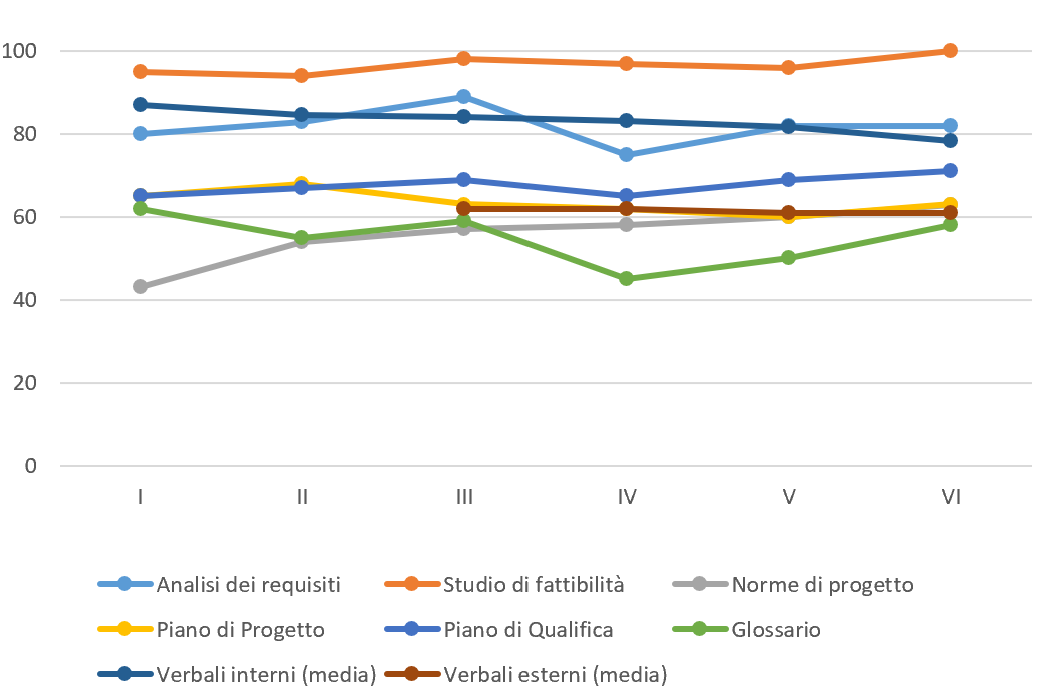
\includegraphics[width=\linewidth]{./img/grafici/2.png}	
	\caption{M15 revisione dei requisiti}	
\end{figure}
\subsubsection{Esito della revisione esterna}
Il gruppo ritiene poco soddisfacenti i risultati della revisione esterna. 
Le correzioni comunicate attraverso colloqui con i committenti e commenti alla valutazione ci hanno permesso di riflettere sui cambiamenti necessari da mettere in atto sia sui nostri prodotti che sul nostro way of working\glo.
Abbiamo quindi deciso di dare più importanza ai ruoli di verificatore e progettista per non ripetere gli errori della precedente revisione e per sopperire alle carenze segnalate.
Questo non si rifletterà con un aumento delle ore nei ruoli individuati, ma con un maggiore impegno da parte dei componenti del gruppo perché migliori la qualità delle ore svolte e non il numero.

\subsection{Revisione di progettazione (RP)}
\subsubsection{Riassunto delle attività di verifica}
In questo periodo abbiamo attuato le verifiche sui documenti, come nel precedente periodo. A queste abbiamo aggiunto le prime verifiche sulla codifica e sulla pianificazione per verificare che lo svolgimento del progetto procedesse senza intoppi.  
\paragraph{Analisi statica dei documenti}
L'analisi statica\glosp dei documenti ha portato alla produzione di una lista degli errori comuni ridotti rispetto alla revisione precedente. Questa lista deve essere aggiornata con le prossime analisi e andrà a facilitare il compito dei verificatori.
\subsubsection{Esiti delle verifiche} 
\paragraph{M01 Scostamento dei requisiti individuati} \mbox{}
\begin{longtable}[H!] {						
		>{}p{50mm}  		
		>{}p{8mm}
		>{}p{8mm}		
		>{}p{8mm}		
		>{}p{8mm}		
		>{}p{8mm}		
		>{}p{8mm}
		>{}p{8mm}
		>{}p{8mm}
		>{}p{8mm}
	}
\rowcolor{gray!50}
\textbf{} & \textbf{I} & \textbf{II} & \textbf{III} & \textbf{IV} & \textbf{V} & \textbf{VI} \TBstrut \\ [2mm]
\textbf{Scostamenti} & 10 & 23 & 29 & 29 & 29 & - \TBstrut \\ [2mm]
	\rowcolor{white}
\caption{M01 revisione di progettazione\glo}
\end{longtable}
\begin{figure}[H] 	
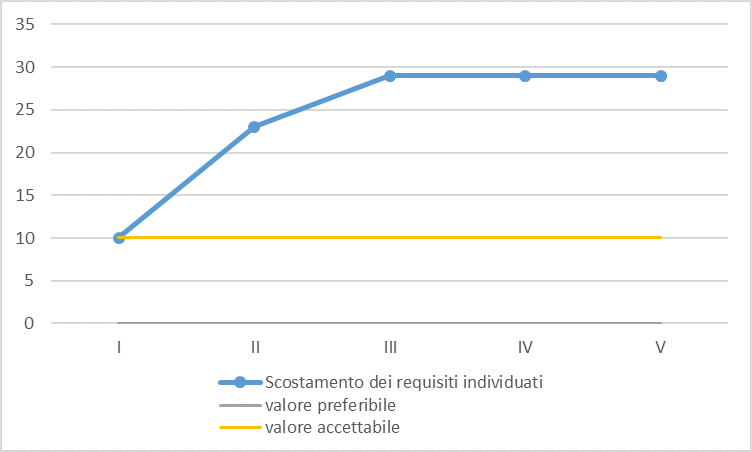
\includegraphics[width=\linewidth]{./img/grafici/RP1.png}	
\caption{M01 revisione di progettazione\glo}	
\end{figure}
\begin{itemize}
	\item \textbf{Valore preferibile}: 0;
	\item \textbf{Valore accettabile}: 10;
	\item \textbf{Considerazioni}: la metrica\glosp non risulta soddisfatta al termine del periodo di progettazione\glo.
\end{itemize}
\paragraph{M02 Numero di parametri per metodo} \mbox{}
\begin{longtable}[H!] {						
		>{}p{50mm}  		
		>{}p{8mm}
		>{}p{8mm}		
		>{}p{8mm}		
		>{}p{8mm}		
		>{}p{8mm}		
		>{}p{8mm}
		>{}p{8mm}
		>{}p{8mm}
		>{}p{8mm}
	}
	\rowcolor{gray!50}
	\textbf{} & \textbf{I} & \textbf{II} & \textbf{III} & \textbf{IV} & \textbf{V} & \textbf{VI} \TBstrut \\ [2mm]
	\textbf{Numero di parametri} & - & - & 3 & 3 & 4 & - \TBstrut \\ [2mm]
	\rowcolor{white}
	\caption{M02 revisione di progettazione\glo}
\end{longtable}
\begin{figure}[H] 	
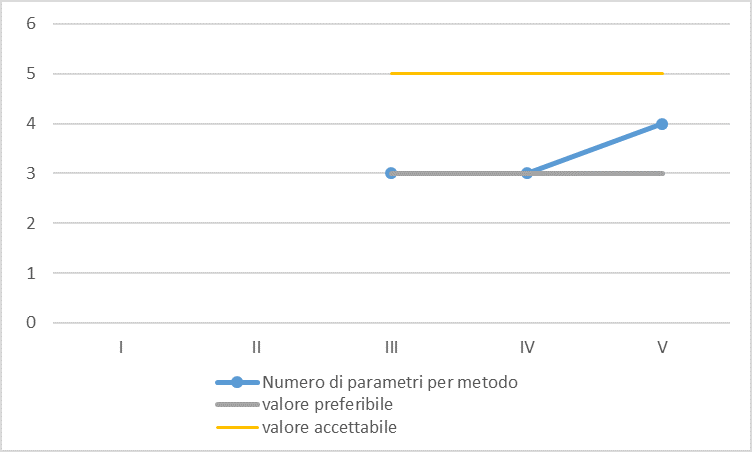
\includegraphics[width=\linewidth]{./img/grafici/RP2.png}	
\caption{M02 revisione di progettazione\glo}	
\end{figure}
\begin{itemize}
	\item \textbf{Valore preferibile}: $\le3$;
	\item \textbf{Valore accettabile}: $\le5$;
	\item \textbf{Considerazioni}: la metrica\glosp risulta soddisfatta al termine del periodo di progettazione\glo.
\end{itemize}
\pagebreak
\paragraph{M03 Numero di metodi per classe} \mbox{}
\begin{longtable}[H!] {						
		>{}p{50mm}  		
		>{}p{8mm}
		>{}p{8mm}		
		>{}p{8mm}		
		>{}p{8mm}		
		>{}p{8mm}		
		>{}p{8mm}
		>{}p{8mm}
		>{}p{8mm}
		>{}p{8mm}
	}
	\rowcolor{gray!50}
	\textbf{} & \textbf{I} & \textbf{II} & \textbf{III} & \textbf{IV} & \textbf{V} & \textbf{VI} \TBstrut \\ [2mm]
	\textbf{Numero di metodi} & - & - & 9 & 9 & 21 & - \TBstrut \\ [2mm]
	\rowcolor{white}
	\caption{M03 revisione di progettazione\glo}
\end{longtable}
\begin{figure}[H] 	
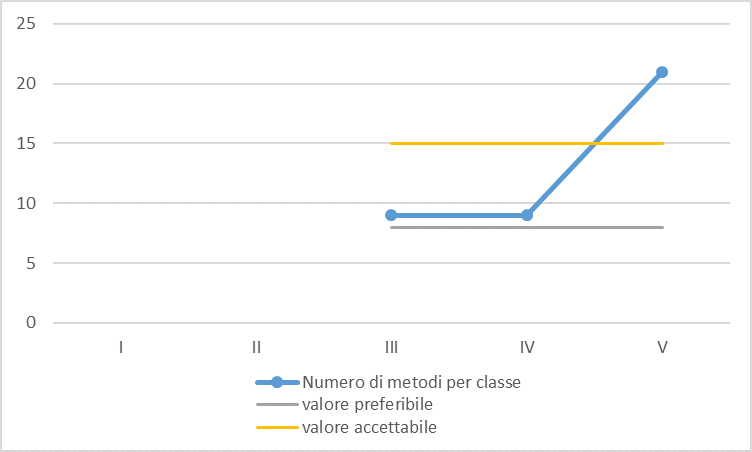
\includegraphics[width=\linewidth]{./img/grafici/RP3.png}	
\caption{M03 revisione di progettazione\glo}	
\end{figure}
\begin{itemize}
	\item \textbf{Valore preferibile}: $\le8$;
	\item \textbf{Valore accettabile}: $\le15$;
	\item \textbf{Considerazioni}: la metrica\glosp non risulta soddisfatta al termine del periodo di progettazione\glo.
\end{itemize}

\paragraph{M15 Indice di Gulpease} \mbox{}
\begin{longtable} {						
		>{}p{50mm}  		
		>{}p{8mm}		
		>{}p{8mm}		
		>{}p{8mm}		
		>{}p{8mm}		
		>{}p{8mm}		
		>{}p{8mm}
		>{}p{8mm}
		>{}p{8mm}
		>{}p{8mm}				
	}			
	\rowcolor{gray!50}
	\textbf{Documento} & \textbf{I} & \textbf{II} & \textbf{III} & \textbf{IV} & \textbf{V} & \textbf{VI} \TBstrut \\ [2mm]
	\textbf{Analisi dei Requisiti} & 3 & 83 & 89 & 75 & 82 & - \TBstrut \\ [2mm]
	\textbf{Norme di Progetto} & 43 & 54 & 57 & 58 & 60 & - \TBstrut \\ [2mm]
	\textbf{Piano di Progetto} & 65 & 68 & 63 & 62 & 60 & - \TBstrut \\ [2mm]
	\textbf{Piano di Qualifica} & 65 & 67 & 69 & 65 & 69 & - \TBstrut \\ [2mm]
	\textbf{Glossario} & 62 & 55 & 59 & 45 & 50 & - \TBstrut \\ [2mm]
	\textbf{Verbali interni (media)} & 87 & 85 & 84 & 83 & 82 & - \TBstrut \\ [2mm]
	\textbf{Verbali esterni (media)} & - & - & 62 & 62 & 61 & - \TBstrut \\ [2mm]
	\rowcolor{white}
	\caption{M15 revisione di progettazione\glo}
\end{longtable}
%\begin{figure}[H] 	
%	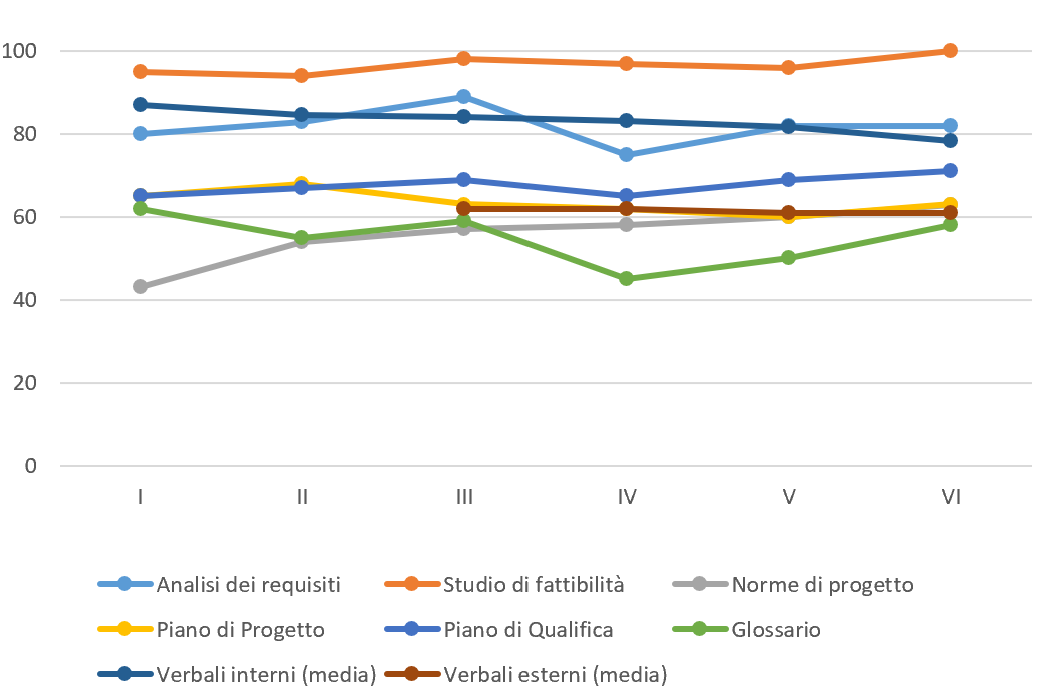
\includegraphics[width=\linewidth]{./img/grafici/2.png}	
%	\caption{M15 revisione di progettazione\glo}	
%\end{figure}
\paragraph{M19 Correttezza ortografica} \mbox{}
\begin{longtable}[H!] {						
		>{}p{50mm}  		
		>{}p{8mm}
		>{}p{8mm}		
		>{}p{8mm}		
		>{}p{8mm}		
		>{}p{8mm}		
		>{}p{8mm}
		>{}p{8mm}
		>{}p{8mm}
		>{}p{8mm}
	}
	\rowcolor{gray!50}
	\textbf{} & \textbf{I} & \textbf{II} & \textbf{III} & \textbf{IV} & \textbf{V} & \textbf{VI} \TBstrut \\ [2mm]
	\textbf{Numero di metodi} & 0 & 1 & 0 & 0 & 0 & - \TBstrut \\ [2mm]
	\rowcolor{white}
	\caption{M19 revisione di progettazione\glo}
\end{longtable}
\begin{figure}[H] 	
	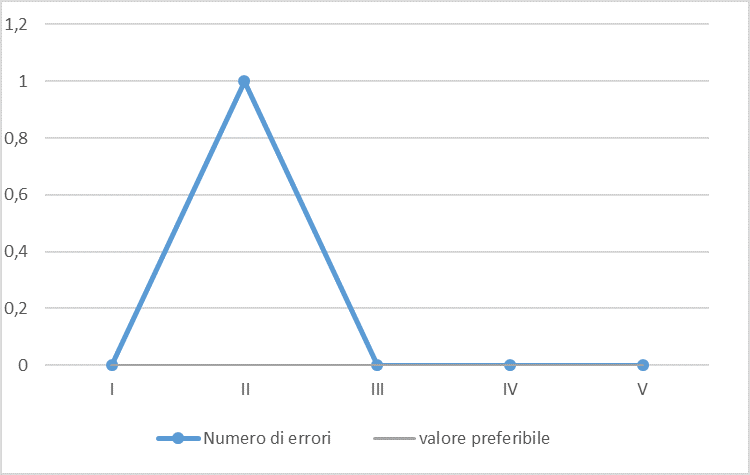
\includegraphics[width=\linewidth]{./img/grafici/RP17.png}	
	\caption{M19 revisione di progettazione\glo}	
\end{figure}
\begin{itemize}
	\item \textbf{Valore preferibile}: $=0$;
	\item \textbf{Valore accettabile}: $=0$;
	\item \textbf{Considerazioni}: la metrica\glosp risulta soddisfatta al termine del periodo di progettazione\glo.
\end{itemize}

\paragraph{M07 Planned value} \mbox{}
\begin{longtable}[H!] {						
		>{}p{38mm}  		
		>{}p{12mm}
		>{}p{12mm}		
		>{}p{12mm}		
		>{}p{12mm}		
		>{}p{12mm}		
		>{}p{12mm}
		>{}p{12mm}
		>{}p{12mm}
		>{}p{12mm}
	}
	\rowcolor{gray!50}
	\textbf{} & \textbf{I} & \textbf{II} & \textbf{III} & \textbf{IV} & \textbf{V} & \textbf{VI} \TBstrut \\ [2mm]
	\textbf{PV} & 800\euro & 1868\euro & 2401\euro & 3068\euro & 3836\euro & - \TBstrut \\ [2mm]
	\rowcolor{white}
	\caption{M07 revisione di progettazione\glo}
\end{longtable}
\begin{figure}[H] 	
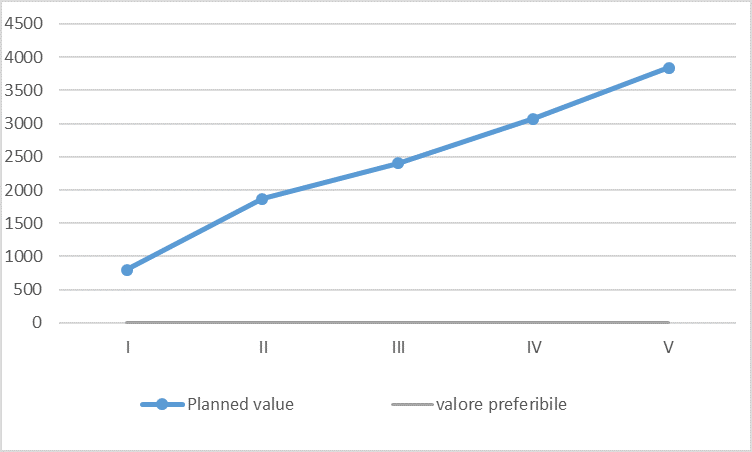
\includegraphics[width=\linewidth]{./img/grafici/RP4.png}	
\caption{M07 revisione di progettazione\glo}	
\end{figure}
\begin{itemize}
	\item \textbf{Valore preferibile}: $\ge0$;
	\item \textbf{Valore accettabile}: $\ge0$;
	\item \textbf{Considerazioni}: la metrica\glosp risulta soddisfatta al termine del periodo di progettazione\glo.
\end{itemize}
\paragraph{M08 Earned value} \mbox{}
\begin{longtable}[H!] {						
		>{}p{38mm}  		
		>{}p{12mm}
		>{}p{12mm}		
		>{}p{12mm}		
		>{}p{12mm}		
		>{}p{12mm}		
		>{}p{12mm}
		>{}p{12mm}
		>{}p{12mm}
		>{}p{12mm}
	}
	\rowcolor{gray!50}
	\textbf{} & \textbf{I} & \textbf{II} & \textbf{III} & \textbf{IV} & \textbf{V} & \textbf{VI} \TBstrut \\ [2mm]
	\textbf{EV} & 650\euro & 1300\euro & 2380\euro & 3050\euro & 3836\euro & - \TBstrut \\ [2mm]
	\rowcolor{white}
	\caption{M08 revisione di progettazione\glo}
\end{longtable}
\begin{figure}[H] 	
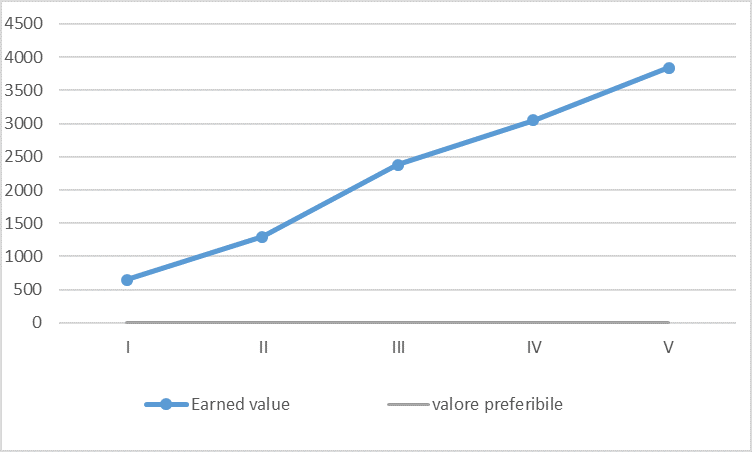
\includegraphics[width=\linewidth]{./img/grafici/RP5.png}	
\caption{M08 revisione di progettazione\glo}	
\end{figure}
\begin{itemize}
	\item \textbf{Valore preferibile}: $\ge0$;
	\item \textbf{Valore accettabile}: $\ge0$;
	\item \textbf{Considerazioni}: la metrica\glosp risulta soddisfatta al termine del periodo di progettazione\glo.
\end{itemize}
\paragraph{M09 Actual cost} \mbox{}
\begin{longtable}[H!] {						
		>{}p{38mm}  		
		>{}p{12mm}
		>{}p{12mm}		
		>{}p{12mm}		
		>{}p{12mm}		
		>{}p{12mm}		
		>{}p{12mm}
		>{}p{12mm}
		>{}p{12mm}
		>{}p{12mm}
	}
	\rowcolor{gray!50}
	\textbf{} & \textbf{I} & \textbf{II} & \textbf{III} & \textbf{IV} & \textbf{V} & \textbf{VI} \TBstrut \\ [2mm]
	\textbf{AC} & 1021\euro & 1982\euro & 2582\euro & 3086\euro & 3836\euro & - \TBstrut \\ [2mm]
	\rowcolor{white}
	\caption{M09 revisione di progettazione\glo}
\end{longtable}
\begin{figure}[H] 	
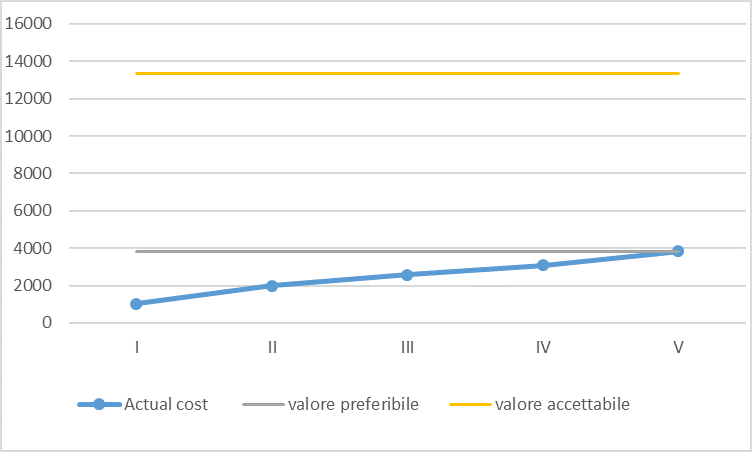
\includegraphics[width=\linewidth]{./img/grafici/RP6.png}	
\caption{M09 revisione di progettazione\glo}	
\begin{itemize}
	\item \textbf{Valore preferibile}: $0\le AC \le PV$;
	\item \textbf{Valore accettabile}: $0 \le AC \le budget \; totale$;
	\item \textbf{Considerazioni}: la metrica\glosp risulta soddisfatta al termine del periodo di progettazione\glo.
\end{itemize}
\end{figure}
\paragraph{M10 Cost performance index} \mbox{}
\begin{longtable}[H!] {						
		>{}p{50mm}  		
		>{}p{8mm}
		>{}p{8mm}		
		>{}p{8mm}		
		>{}p{8mm}		
		>{}p{8mm}		
		>{}p{8mm}
		>{}p{8mm}
		>{}p{8mm}
		>{}p{8mm}
	}
	\rowcolor{gray!50}
	\textbf{} & \textbf{I} & \textbf{II} & \textbf{III} & \textbf{IV} & \textbf{V} & \textbf{VI} \TBstrut \\ [2mm]
	\textbf{CPI} & 0,64 & 0,66 & 0,92 & 0,99 & 1 & - \TBstrut \\ [2mm]
	\rowcolor{white}
	\caption{M10 revisione di progettazione\glo}
\end{longtable}
\begin{figure}[H] 	
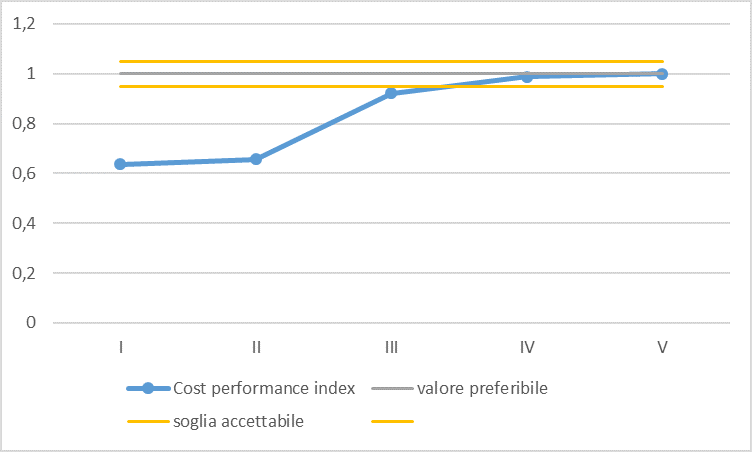
\includegraphics[width=\linewidth]{./img/grafici/RP7.png}	
\caption{M10 revisione di progettazione\glo}	
\end{figure}
\begin{itemize}
	\item \textbf{Valore preferibile}: $=1$;
	\item \textbf{Valore accettabile}: $0.95 \le CPI \le 1.05$;
	\item \textbf{Considerazioni}: la metrica\glosp risulta soddisfatta al termine del periodo di progettazione\glo.
\end{itemize}
\paragraph{M11 Schedule performance index} \mbox{}
\begin{longtable}[H!] {						
		>{}p{50mm}  		
		>{}p{8mm}
		>{}p{8mm}		
		>{}p{8mm}		
		>{}p{8mm}		
		>{}p{8mm}		
		>{}p{8mm}
		>{}p{8mm}
		>{}p{8mm}
		>{}p{8mm}
	}
	\rowcolor{gray!50}
	\textbf{} & \textbf{I} & \textbf{II} & \textbf{III} & \textbf{IV} & \textbf{V} & \textbf{VI} \TBstrut \\ [2mm]
	\textbf{SPI} & 0,81 & 0,69 & 0,99 & 0,99 & 1 & - \TBstrut \\ [2mm]
	\rowcolor{white}
	\caption{M11 revisione di progettazione\glo}
\end{longtable}
\begin{figure}[H] 	
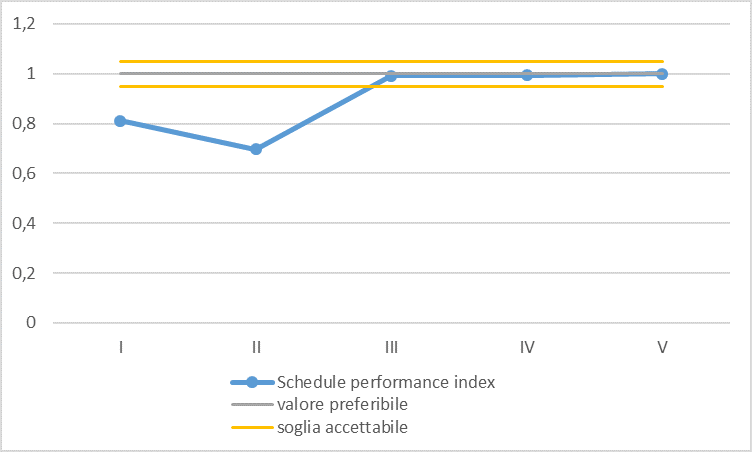
\includegraphics[width=\linewidth]{./img/grafici/RP8.png}	
\caption{M11 revisione di progettazione\glo}	
\end{figure}
\begin{itemize}
	\item \textbf{Valore preferibile}: $=1$;
	\item \textbf{Valore accettabile}: $0.95 \le SPI \le 1.05$;
	\item \textbf{Considerazioni}: la metrica\glosp risulta soddisfatta al termine del periodo di progettazione\glo.
\end{itemize}
\paragraph{M12 Estimated cost at compltion} \mbox{}
\begin{longtable}[H!] {						
		>{}p{38mm}  		
		>{}p{12mm}
		>{}p{12mm}		
		>{}p{12mm}		
		>{}p{12mm}		
		>{}p{12mm}		
		>{}p{12mm}
		>{}p{12mm}
		>{}p{12mm}
		>{}p{12mm}
	}
	\rowcolor{gray!50}
	\textbf{} & \textbf{I} & \textbf{II} & \textbf{III} & \textbf{IV} & \textbf{V} & \textbf{VI} \TBstrut \\ [2mm]
	\textbf{EAC} & 20955\euro & 20340\euro & 14473\euro & 13498\euro & 13341\euro & - \TBstrut \\ [2mm]
	\rowcolor{white}
	\caption{M12 revisione di progettazione\glo}
\end{longtable}
\begin{figure}[H] 	
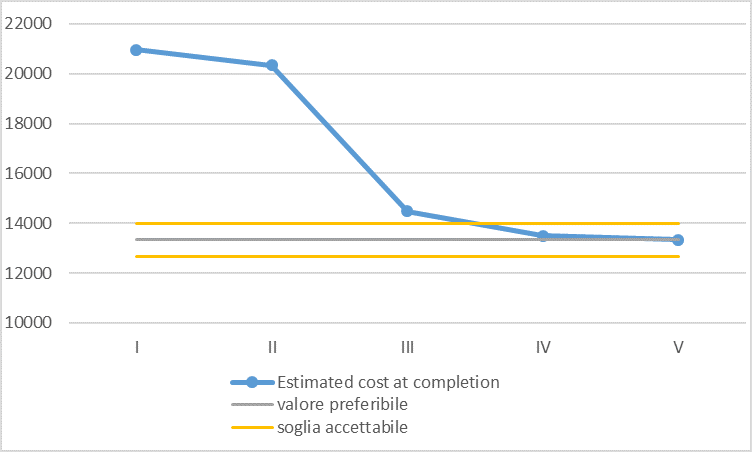
\includegraphics[width=\linewidth]{./img/grafici/RP9.png}	
\caption{M12 revisione di progettazione\glo}	
\end{figure}
\begin{itemize}
	\item \textbf{Valore preferibile}: pari a quanto preventivato;
	\item \textbf{Valore accettabile}: $preventivo-5\% \le EAC \le preventivo+5\%$;
	\item \textbf{Considerazioni}: la metrica\glosp risulta soddisfatta al termine del periodo di progettazione\glo.
\end{itemize}
\paragraph{M13 Schedule at completion} \mbox{}
\begin{longtable}[H!] {						
	>{}p{18mm}  		
	>{}p{16mm}
	>{}p{16mm}		
	>{}p{16mm}		
	>{}p{16mm}		
	>{}p{16mm}		
	>{}p{16mm}
	>{}p{16mm}
	>{}p{16mm}
	>{}p{16mm}
	}
	\rowcolor{gray!50}
	\textbf{} & \textbf{I} & \textbf{II} & \textbf{III} & \textbf{IV} & \textbf{V} & \textbf{VI} \TBstrut \\ [2mm]
	\textbf{SAC} & 879 ore & 1026 ore & 720 ore & 718 ore & 714 ore & - \TBstrut \\ [2mm]
	\rowcolor{white}
	\caption{M13 revisione di progettazione\glo}
\end{longtable}
\begin{figure}[H] 	
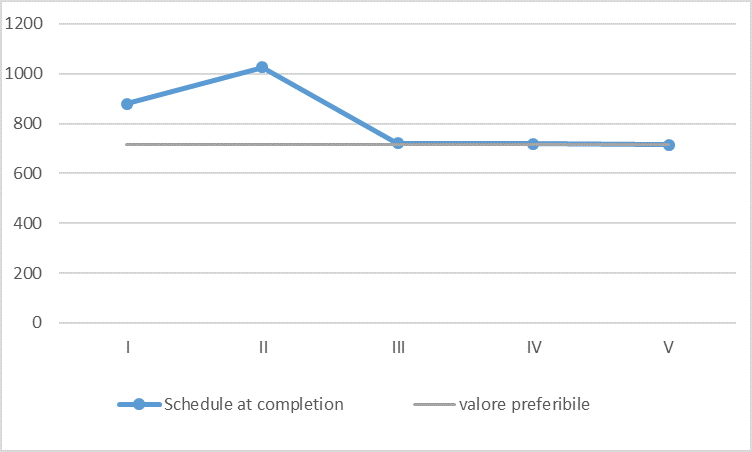
\includegraphics[width=\linewidth]{./img/grafici/RP10.png}	
\caption{M13 revisione di progettazione\glo}	
\end{figure}
\begin{itemize}
	\item \textbf{Valore preferibile}: pari a quanto preventivato;
	\item \textbf{Valore accettabile}: pari a quanto preventivato;
	\item \textbf{Considerazioni}: la metrica\glosp risulta soddisfatta al termine del periodo di progettazione\glo.
\end{itemize}
\paragraph{M14 Rischi non preventivati} \mbox{}
\begin{longtable}[H!] {						
		>{}p{50mm}  		
		>{}p{8mm}
		>{}p{8mm}		
		>{}p{8mm}		
		>{}p{8mm}		
		>{}p{8mm}		
		>{}p{8mm}
		>{}p{8mm}
		>{}p{8mm}
		>{}p{8mm}
	}
	\rowcolor{gray!50}
	\textbf{} & \textbf{I} & \textbf{II} & \textbf{III} & \textbf{IV} & \textbf{V} & \textbf{VI} \TBstrut \\ [2mm]
	\textbf{Rischi} & 0 & 0 & 0 & 0 & 0 & - \TBstrut \\ [2mm]
	\rowcolor{white}
	\caption{M14 revisione di progettazione\glo}
\end{longtable}
\begin{figure}[H] 	
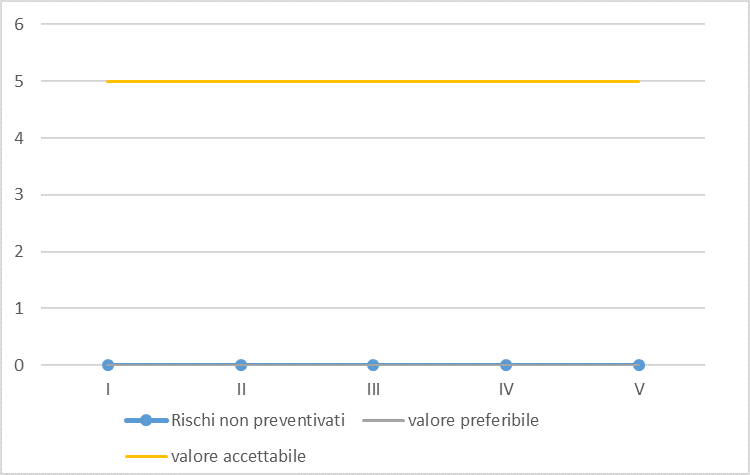
\includegraphics[width=\linewidth]{./img/grafici/RP11.png}	
\caption{M14 revisione di progettazione\glo}	
\end{figure}
\begin{itemize}
	\item \textbf{Valore preferibile}: $=0$;
	\item \textbf{Valore accettabile}: $\le 5$;
	\item \textbf{Considerazioni}: la metrica\glosp risulta soddisfatta al termine del periodo di progettazione\glo.
\end{itemize}
\paragraph{M06 Tempo medio risoluzione errori} \mbox{}
\begin{longtable}[H!] {						
		>{}p{38mm}  		
		>{}p{12mm}
		>{}p{12mm}		
		>{}p{12mm}		
		>{}p{12mm}		
		>{}p{12mm}		
		>{}p{12mm}
		>{}p{12mm}
		>{}p{12mm}
		>{}p{12mm}
	}
	\rowcolor{gray!50}
	\textbf{} & \textbf{I} & \textbf{II} & \textbf{III} & \textbf{IV} & \textbf{V} & \textbf{VI} \TBstrut \\ [2mm]
	\textbf{Tempo medio} & 15min & 134min & 122min & 110min & 104min & - \TBstrut \\ [2mm]
	\rowcolor{white}
	\caption{M06 revisione di progettazione\glo}
\end{longtable}
\begin{figure}[H] 	
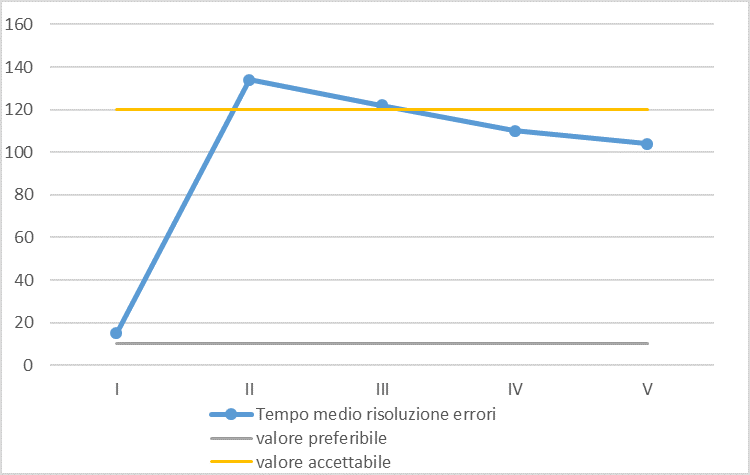
\includegraphics[width=\linewidth]{./img/grafici/RP12.png}	
\caption{M06 revisione di progettazione\glo}	
\end{figure}
\begin{itemize}
	\item \textbf{Valore preferibile}: $\le10minuti$;
	\item \textbf{Valore accettabile}: $\le120minuti$;
	\item \textbf{Considerazioni}: la metrica\glosp risulta soddisfatta al termine del periodo di progettazione\glo.
\end{itemize}
\paragraph{M16 Percentuale di requisiti obbligatori soddisfatti} \mbox{}
\begin{longtable}[H!] {						
		>{}p{50mm}  		
		>{}p{8mm}
		>{}p{8mm}		
		>{}p{8mm}		
		>{}p{8mm}		
		>{}p{8mm}		
		>{}p{8mm}
		>{}p{8mm}
		>{}p{8mm}
		>{}p{8mm}
	}
	\rowcolor{gray!50}
	\textbf{} & \textbf{I} & \textbf{II} & \textbf{III} & \textbf{IV} & \textbf{V} & \textbf{VI} \TBstrut \\ [2mm]
	\textbf{PROS} & - & - & 32\% & 53\% & 53\% & - \TBstrut \\ [2mm]
	\rowcolor{white}
	\caption{M16 revisione di progettazione\glo}
\end{longtable}
\begin{figure}[H] 	
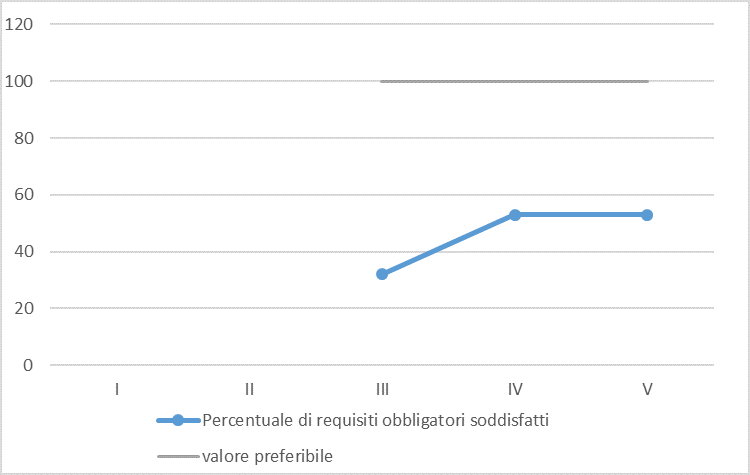
\includegraphics[width=\linewidth]{./img/grafici/RP13.png}	
\caption{M16 revisione di progettazione\glo}	
\end{figure}
\begin{itemize}
	\item \textbf{Valore preferibile}: $=100\%$;
	\item \textbf{Valore accettabile}: $=100\%$;
	\item \textbf{Considerazioni}: la metrica\glosp risulta non soddisfatta al termine del periodo di progettazione\glo.
\end{itemize}
\paragraph{M17 Percentuale di requisiti desiderabili soddisfatti} \mbox{}
\begin{longtable}[H!] {						
		>{}p{50mm}  		
		>{}p{8mm}
		>{}p{8mm}		
		>{}p{8mm}		
		>{}p{8mm}		
		>{}p{8mm}		
		>{}p{8mm}
		>{}p{8mm}
		>{}p{8mm}
		>{}p{8mm}
	}
	\rowcolor{gray!50}
	\textbf{} & \textbf{I} & \textbf{II} & \textbf{III} & \textbf{IV} & \textbf{V} & \textbf{VI} \TBstrut \\ [2mm]
	\textbf{PRDS} & - & - & 0\% & 0\% & 0\% & - \TBstrut \\ [2mm]
	\rowcolor{white}
	\caption{M17 revisione di progettazione\glo}
\end{longtable}
\begin{figure}[H] 	
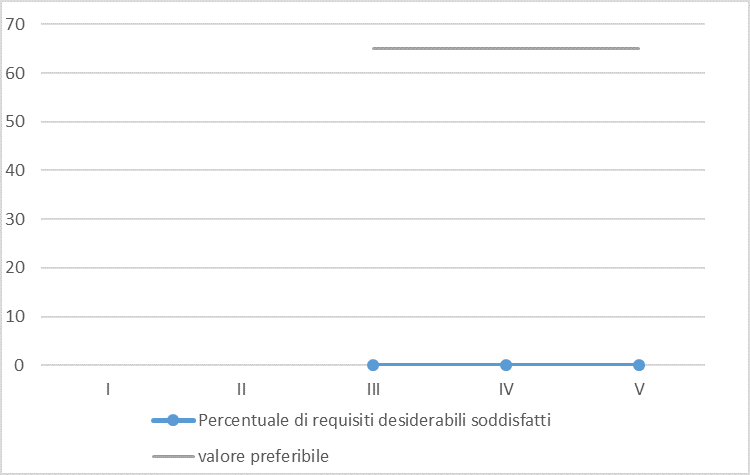
\includegraphics[width=\linewidth]{./img/grafici/RP14.png}	
\caption{M17 revisione di progettazione\glo}	
\end{figure}
\begin{itemize}
	\item \textbf{Valore preferibile}: $\ge 65\%$;
	\item \textbf{Valore accettabile}: $\ge 0\%$;
	\item \textbf{Considerazioni}: la metrica\glosp risulta soddisfatta al termine del periodo di progettazione\glo.
\end{itemize}
\paragraph{M18 Percentuale di requisiti opzionali soddisfatti} \mbox{}
\begin{longtable}[H!] {						
		>{}p{50mm}  		
		>{}p{8mm}
		>{}p{8mm}		
		>{}p{8mm}		
		>{}p{8mm}		
		>{}p{8mm}		
		>{}p{8mm}
		>{}p{8mm}
		>{}p{8mm}
		>{}p{8mm}
	}
	\rowcolor{gray!50}
	\textbf{} & \textbf{I} & \textbf{II} & \textbf{III} & \textbf{IV} & \textbf{V} & \textbf{VI} \TBstrut \\ [2mm]
	\textbf{PROpS} & - & - & 0\% & 0\% & 0\% & - \TBstrut \\ [2mm]
	\rowcolor{white}
	\caption{M18 revisione di progettazione\glo}
\end{longtable}
\begin{figure}[H] 	
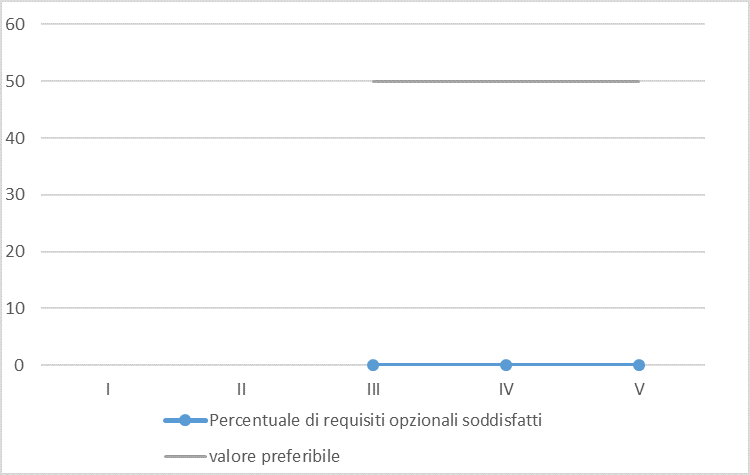
\includegraphics[width=\linewidth]{./img/grafici/RP15.png}	
\caption{M18 revisione di progettazione\glo}	
\end{figure}
\begin{itemize}
	\item \textbf{Valore preferibile}: $\ge50\%$;
	\item \textbf{Valore accettabile}: $\ge0\%$;
	\item \textbf{Considerazioni}: la metrica\glosp risulta soddisfatta al termine del periodo di progettazione\glo.
\end{itemize}
\paragraph{M05 Percentuale bug sistemati} \mbox{}
\begin{longtable}[H!] {						
		>{}p{50mm}  		
		>{}p{8mm}
		>{}p{8mm}		
		>{}p{8mm}		
		>{}p{8mm}		
		>{}p{8mm}		
		>{}p{8mm}
		>{}p{8mm}
		>{}p{8mm}
		>{}p{8mm}
	}
	\rowcolor{gray!50}
	\textbf{} & \textbf{I} & \textbf{II} & \textbf{III} & \textbf{IV} & \textbf{V} & \textbf{VI} \TBstrut \\ [2mm]
	\textbf{Bug sistemati} & - & - & 0\% & 30\% & 40\% & - \TBstrut \\ [2mm]
	\rowcolor{white}
	\caption{M05 revisione di progettazione\glo}
\end{longtable}
\begin{figure}[H] 	
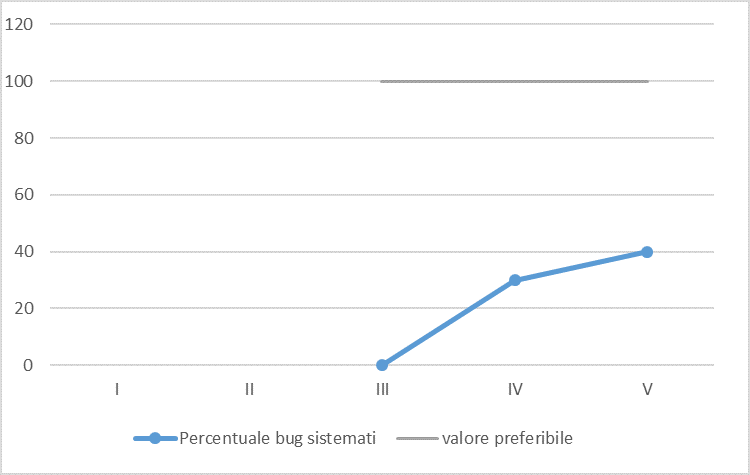
\includegraphics[width=\linewidth]{./img/grafici/RP16.png}	
\caption{M05 revisione di progettazione\glo}	
\end{figure}
\begin{itemize}
	\item \textbf{Valore preferibile}: $=100\%$;
	\item \textbf{Valore accettabile}: $=100\%$;
	\item \textbf{Considerazioni}: la metrica\glosp risulta non soddisfatta al termine del periodo di progettazione\glo.
\end{itemize}
\paragraph{M04 Percentuale di metriche soddisfatte} \mbox{}
\begin{longtable}[H!] {						
		>{}p{50mm}  		
		>{}p{8mm}
		>{}p{8mm}		
		>{}p{8mm}		
		>{}p{8mm}		
		>{}p{8mm}		
		>{}p{8mm}
		>{}p{8mm}
		>{}p{8mm}
		>{}p{8mm}
	}
	\rowcolor{gray!50}
	\textbf{} & \textbf{I} & \textbf{II} & \textbf{III} & \textbf{IV} & \textbf{V} & \textbf{VI} \TBstrut \\ [2mm]
	\textbf{Numero di metodi} & - & - & 3 & 3 & 3 & - \TBstrut \\ [2mm]
	\rowcolor{white}
	\caption{M04 revisione di progettazione\glo}
\end{longtable}
%\begin{figure}[H] 	
%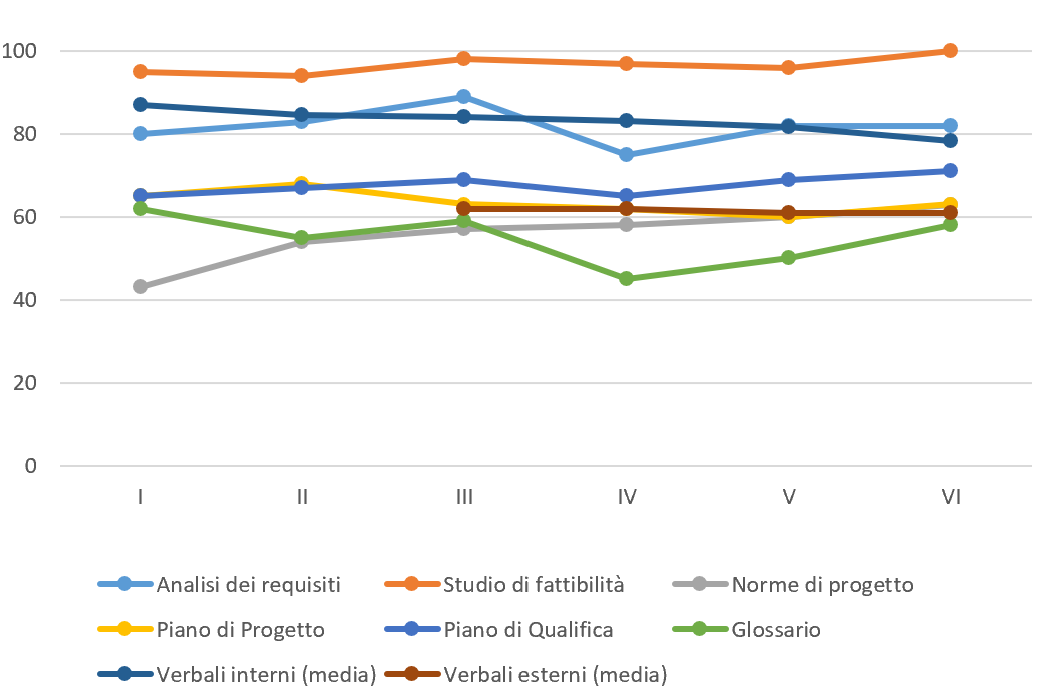
\includegraphics[width=\linewidth]{./img/grafici/2.png}	
%\caption{M04 revisione di progettazione\glo}	
%\end{figure}


















\subsubsection{Revisioni generali}\mbox{}
\begin{longtable} {						
		>{}p{50mm}  		
		>{}p{8mm}		
		>{}p{8mm}		
		>{}p{8mm}		
		>{}p{8mm}		
		>{}p{8mm}		
		>{}p{8mm}
		>{}p{8mm}				
	}			
	\rowcolor{gray!50}
	\textbf{Metrica} & \textbf{RR} & \textbf{RP} & \textbf{RQ} & \textbf{RA} \TBstrut \\ [2mm]
	\textbf{Indice di Gulpease (media)} & 82 & - & - & - \TBstrut \\ [2mm]
	\textbf{M01} & 100 & - & - & - \TBstrut \\ [2mm]
	\textbf{Norme di Progetto} & 63 & - & - & - \TBstrut \\ [2mm]
	\textbf{Piano di Progetto} & 63 & - & - & - \TBstrut \\ [2mm]
	\textbf{Piano di Qualifica} & 71 & - & - & - \TBstrut \\ [2mm]
	\textbf{Glossario} & 58 & - & - & - \TBstrut \\ [2mm]
	\textbf{Verbali interni (media)} & 78 & - & - & - \TBstrut \\ [2mm]
	\textbf{Verbali esterni (media)}& 61 & - & - & - \TBstrut \\ [2mm]
	\rowcolor{white}
	\caption{Indice di Gulpease}
\end{longtable}
\begin{figure}[H] 	
	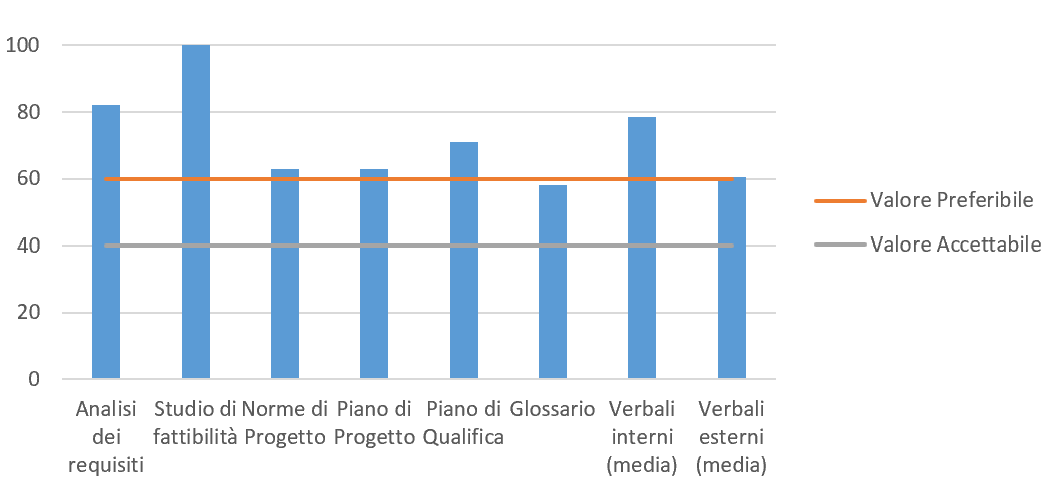
\includegraphics[width=\linewidth]{./img/grafici/1.png}	
	\caption{Indice di Gulpease}	
\end{figure}
	\pagebreak
	\section{Valutazioni per il miglioramento} 
Lo scopo di questa sezione è di tracciare e riportare i problemi sorti durante il lavoro svolto dal gruppo per individuare delle soluzioni efficaci ed efficienti che permettano di migliorare la collaborazione e aumentare la qualità dei prodotti\glosp realizzati.
\\L'individuazione e l'analisi delle criticità e dei problemi è svolta dagli stessi membri del gruppo. Ognuno è incaricato di appuntarsi le criticità e i problemi che riscontra in modo che possano essere discussi nella riunione di gruppo successiva. Ad ogni riunione avviene quindi un confronto in cui si discute dei possibili miglioramenti da applicare per eliminare i problemi esistenti nel modo più efficace ed efficiente. Per problemi di particolare gravità o urgenza si organizzano delle riunioni apposite il prima possibile.
\\ \\Sono quindi tracciati i problemi riscontrati nei seguenti ambiti:

\begin{itemize}
	\item \textbf{Organizzazione}: problemi riguardanti l'organizzazione del lavoro e della comunicazione all'interno del gruppo;
	\item \textbf{Ruoli}: problemi riguardanti il corretto funzionamento dei ruoli;
	\item \textbf{Strumenti}: problemi riguardanti gli strumenti di lavoro utilizzati.
\end{itemize}

\subsection{Valutazioni sull'organizzazione}
	\subsubsection{Organizzazione incontri}
		\begin{itemize}
			\item \textbf{Descrizione problema}: è stata riscontrata una certa difficoltà nell'organizzare incontri frequenti a cui fossero presenti tutti i membri del gruppo;
			\item \textbf{Soluzione individuata}: si è deciso di dare priorità a riunioni via Skype, utilizzando la condivisione degli schermi per poter collaborare in modo efficace ed efficiente.
		\end{itemize}
		\subsubsection{Comunicazione via chat}
			\begin{itemize}
			\item \textbf{Descrizione problema}: la comunicazione via chat fra i membri del gruppo si è rivelata non sufficientemente collaborativa e tempestiva;
			\item \textbf{Soluzione individuata}: si è deciso, di comune accordo, di impegnarsi nell'essere più partecipi e propositivi nelle conversazioni. Come aiuto ogni membro del gruppo ha installato le apposite applicazioni di messaggistica abilitando notifiche prioritarie per i messaggi del gruppo.
			\end{itemize}
\subsection{Valutazioni sui ruoli}
	\subsubsection{Ripartizione equa delle attività da parte del responsabile}
	\begin{itemize}
		\item \textbf{Descrizione problema}: a causa dell'inesperienza dei membri del gruppo, il carico di lavoro non è sempre stato suddiviso in modo equo dal responsabile;
		\item \textbf{Soluzione individuata}: si è iniziato il prima possibile a monitorare il lavoro tramite il sistema di ticketing GitHub, così grazie alle project board e all'assegnazione delle attività il responsabile è riuscito a ripartizionare e monitorare in modo sempre migliore il carico di lavoro.
	\end{itemize}
	\subsubsection{Pianificazione corretta delle milestone da parte del responsabile}
	\begin{itemize}
	\item \textbf{Descrizione problema}: a causa dell'inesperienza dei membri del gruppo, le milestone non sono sempre state fissate dal responsabile in date adeguate;
	\item \textbf{Soluzione individuata}: si è iniziato il prima possibile ad utilizzare le milestone ed i ticket su GitHub, così grazie alle project board il responsabile è riuscito a valutare in modo migliore i collocamenti delle milestone.
	\end{itemize}
	\subsubsection{Rapporto fra verificatori ed analisti}
		\begin{itemize}
			\item \textbf{Descrizione problema}: nelle fasi iniziali, dato l'ancora scarso affiatamento fra i membri del gruppo, si è instaurata una situazione allievo-maestro fra analisti e verificatori;
			\item \textbf{Soluzione individuata}: si è deciso che le prime verifiche dovevano essere collettive, facendo partecipare più membri del gruppo alla verifica dei documenti favorendo così una discussione costruttiva.
		\end{itemize}
	\subsubsection{Amministratore}
		\begin{itemize}
			\item \textbf{Descrizione problema}: il problema principale dell'amministratore è stato quello di aggiornare in modo tempestivo le \textit{Norme di Progetto} per normare le attività del gruppo senza rallentarle;
			\item \textbf{Soluzione individuata}: si è lavorato maggiormente a livello di pianificazione e se necessario è stato dato maggiore supporto all'amministratore durante l'aggiornamento delle norme.
		\end{itemize}
\subsection{Valutazioni sugli strumenti}
	\subsubsection{\LaTeX}
		\begin{itemize}
			\item \textbf{Descrizione problema}: la scarsa conoscenza di \LaTeX\xspace da parte dei membri del gruppo ha reso difficile avere una struttura uniforme e concorde in tutte le parti dei documenti;
			\item \textbf{Soluzione individuata}: si è creato il prima possibile un template \LaTeX\xspace stabile che contenesse le sezioni base e la struttura generale dei documenti. Inoltre i membri del gruppo più esperti hanno istruito gli altri sulle funzionalità di \LaTeX.
		\end{itemize}
	\subsubsection{TeXStudio}
		\begin{itemize}
			\item \textbf{Descrizione problema}: il controllo linguistico di TeXStudio non è disponibile di default in italiano ed alcuni membri del gruppo hanno avuto difficoltà ad installarlo, anche a causa dei differenti sistemi operativi;
			\item \textbf{Soluzione individuata}: sono stati incaricati due membri del gruppo affinché trovassero una soluzione per Microsoft Windows ed una per Linux. Una volta individuate le soluzioni hanno istruito gli altri membri del gruppo su come installare e configurare il correttore linguistico in italiano.
		\end{itemize}
	\subsubsection{Git}
		\begin{itemize}
			\item \textbf{Descrizione problema}: la scarsa esperienza nell'uso di Git ed in particolare dei branch ha inizialmente causato confusione e conflitti frequenti sui file;
			\item \textbf{Soluzione individuata}: si è deciso di organizzare un piccolo corso in cui i membri del gruppo più esperti hanno spiegato tramite esempi ed esercizi l'uso del sistema di versionamento\glosp Git e dei branch. 
		\end{itemize}
	\subsubsection{GitHub}
		\begin{itemize}
		\item \textbf{Descrizione problema}: la scarsa esperienza nell'uso di GitHub ed in particolare delle pull-request ha inizialmente causato confusione e rallentato le attività di analisi e verifica;
		\item \textbf{Soluzione individuata}: si è deciso di organizzare un piccolo corso in cui i membri del gruppo più esperti hanno spiegato tramite esempi ed esercizi l'uso delle pull-request su GitHub. 
		\end{itemize}
	\subsubsection{Slack}
		\begin{itemize}
			\item \textbf{Descrizione problema}: la scarsa esperienza nell'uso di Slack ed in particolare dei thread e dei canali ha causato difficoltà di comunicazione e disordine nelle conversazioni;
			\item \textbf{Soluzione individuata}: i membri più esperti del gruppo hanno istruito gli altri componenti ed hanno incentivato l'uso di thread e canali, andando a correggere i casi in cui la comunicazione non avveniva in modo corretto. 
		\end{itemize}
	
	%Input del file "decision_table" della cartella locale "res/"
	%% \textbf = grassetto; \Large = font più grande
% \rowcolors{quanti colori alternare}{colore numero riga pari}{colore numero riga dispari}: colori alternati per riga
% \rowcolor{color}: cambia colore di una riga
% p{larghezza colonna}: p è un tipo di colonna di testo verticalmente allineata sopra, ci sarebbe anche m che è centrata a metà ma non è precisa per questo utilizzo TBStrut; la sintassi >{\centering} indica che il contenuto della colonna dovrà essere centrato
% \TBstrut fa parte di alcuni comandi che ho inserito in config.tex che permetto di aggiungere un po' di padding al testo
% \\ [2mm] : questra scrittura indica che lo spazio dopo una break line deve essere di 2mm

%\setcounter{secnumdepth}{0}
%\hfill \break
%\textbf{\Large{Diario delle modifiche}} \\
\section{Riepilogo tracciamenti}
\rowcolors{2}{gray!25}{gray!15}
\begin{longtable} {
		>{\centering}p{17mm} 
		%>{\centering}p{19.5mm}
		%>{\centering}p{24mm} 
		%>{\centering}p{24mm} 
		>{}p{120mm}}
	\rowcolor{gray!50}
	\textbf{Codice} & \multicolumn{1}{c}{\textbf{Decisione}} \\%\textbf{Decisione} \\ %\TBstrut \\
	VI\_1.1 & Scelto \textit{VRAM Software} come nome del gruppo. \TBstrut \\ [2mm]
	VI\_1.1 & Scelto \textit{VRAM Software} come nome del gruppo. \TBstrut \\ [2mm]
	VI\_1.1 & Scelto \textit{VRAM Software} come nome del gruppo. \TBstrut \\ [2mm]
	
\end{longtable} %Tabella delle decisioni (solo per i verbali)
\end{document}